\chapter{User Interface Design} \label{ui}

This third chapter is about the frontend interfaces the users will use for accessing and interacting with the two systems. For every system, there is a brief  presentation of all the main interfaces they are composed of, and then, thanks to the use of flow diagrams, the navigation flow is presented.\medskip

These represent only the interfaces used by the end users of the two systems, the pages for the system administrators are not presented here, since their views are similar to these or consist only of a list of employees with the possibility to add or remove them (which is especially true in the CPMS).\medskip

Moreover, these interfaces are presented only in day/light mode for better readability, but in real-case scenarios, they adapt to the user's (or browser's) preferred theme, so they come also with a night/dark mode.

\section{eMSP}

The eMSP is the system that interacts with the end user of the whole system: the consumer. In this section, the only presented mockups are the ones of the mobile application. The ones available from the browser are the same, with the only difference being that in the case of a landscape design (which is more common on desktop/personal computers), the elements of the interfaces are organized in a slightly different way to better adapt to the display.

\subsection{Interfaces design}

Here are presented all the mockups of the pages of the mobile application of the eMSP. The mobile application is available on all the main application stores for mobile phones available nowadays, like \textit{App Store} (Apple), \textit{Google Play Store} (Google), and \textit{AppGallery} (Huawei). The browser version is slightly different since it's usually used on a landscape device.

\pagebreak

\paragraph{Login and signup} When the user first opens the application or the personal area of the eMSP website, he is prompted to log into the application, but if the user doesn't still have an account, there is the possibility to go to the signup page (or registration page) where he is asked to insert all of his data. The interface also offers the possibility to display (or to hide) the password and to display a date picker to easily insert the birthdate.

\begin{figure}[h!]
    \centering
    \begin{minipage}{0.49\textwidth}
        \centering
        \fbox{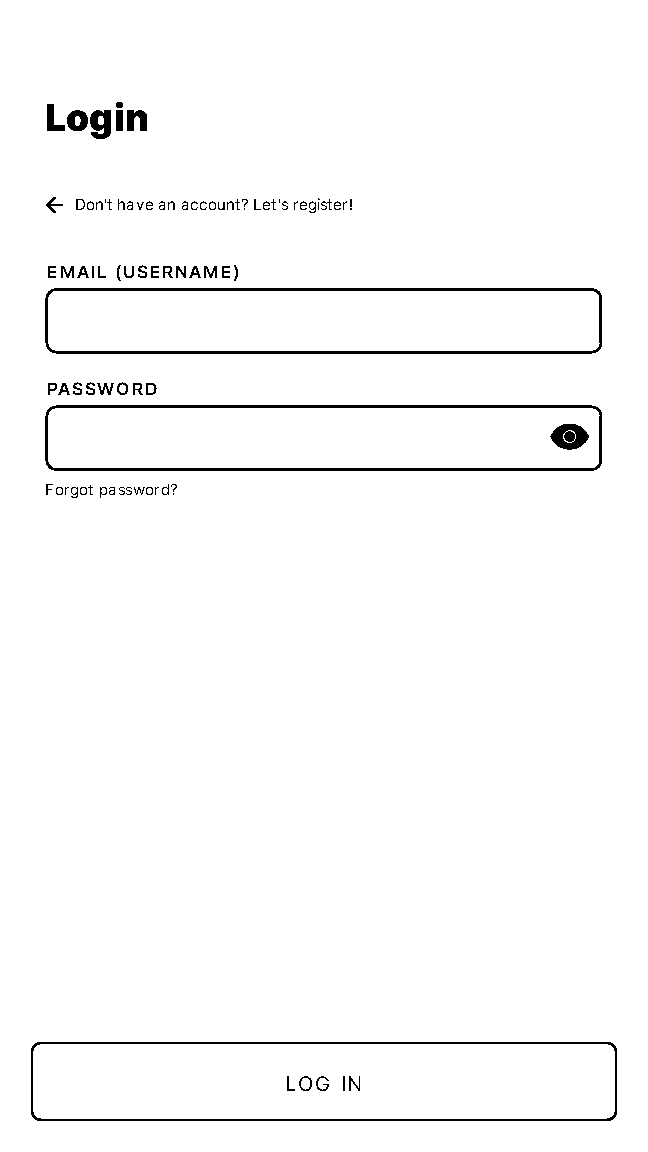
\includegraphics[width=\textwidth]{images/mockups/emsp/signup_login/login}}
        \caption{login page.}
    \end{minipage}
    \hfill
    \begin{minipage}{0.49\textwidth}
        \centering
        \fbox{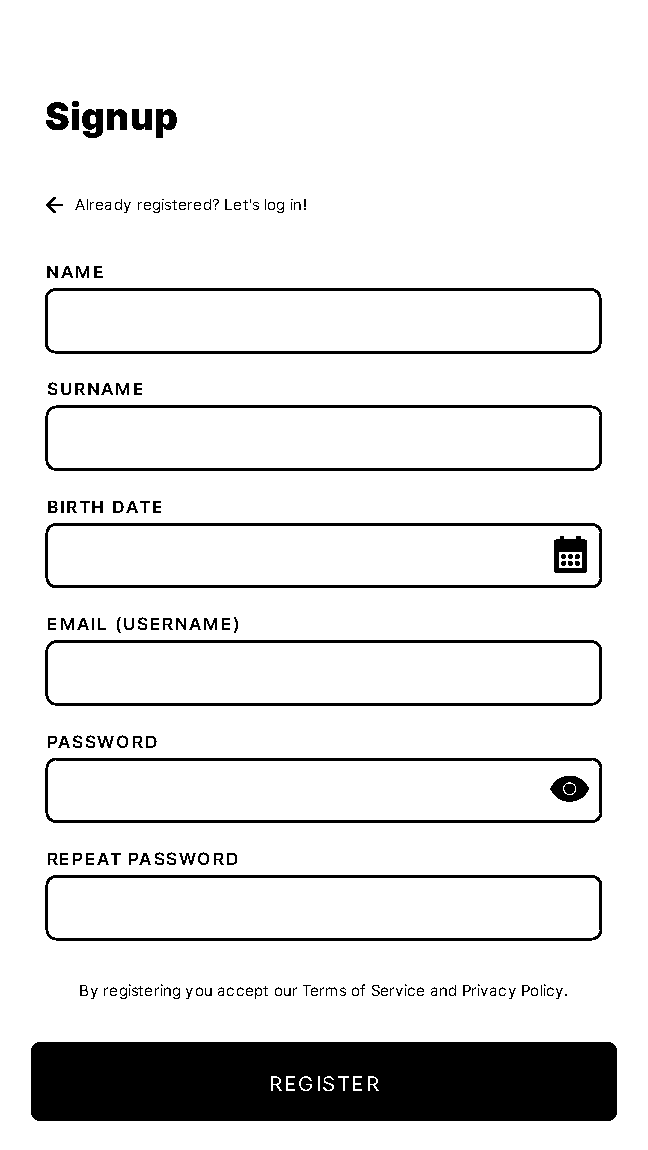
\includegraphics[width=\textwidth]{images/mockups/emsp/signup_login/signup}}
        \caption{signup (registration) page.}
    \end{minipage}
\end{figure}

\pagebreak

\paragraph{Post registration actions} After the uses registers to the application, the system sends him/her an email with a link for activating the account. Once the user clicks on it, s/he is sent to the login page where a popup tells the user that his/her registration ended up successfully. After closing the banner, the user can log into the application, and since it's the first login, the home page is displayed and s/he is asked whether to use any logged-in device for sending notifications or the associated email address.

\begin{figure}[h!]
    \begin{minipage}{0.49\textwidth}
        \centering
        \fbox{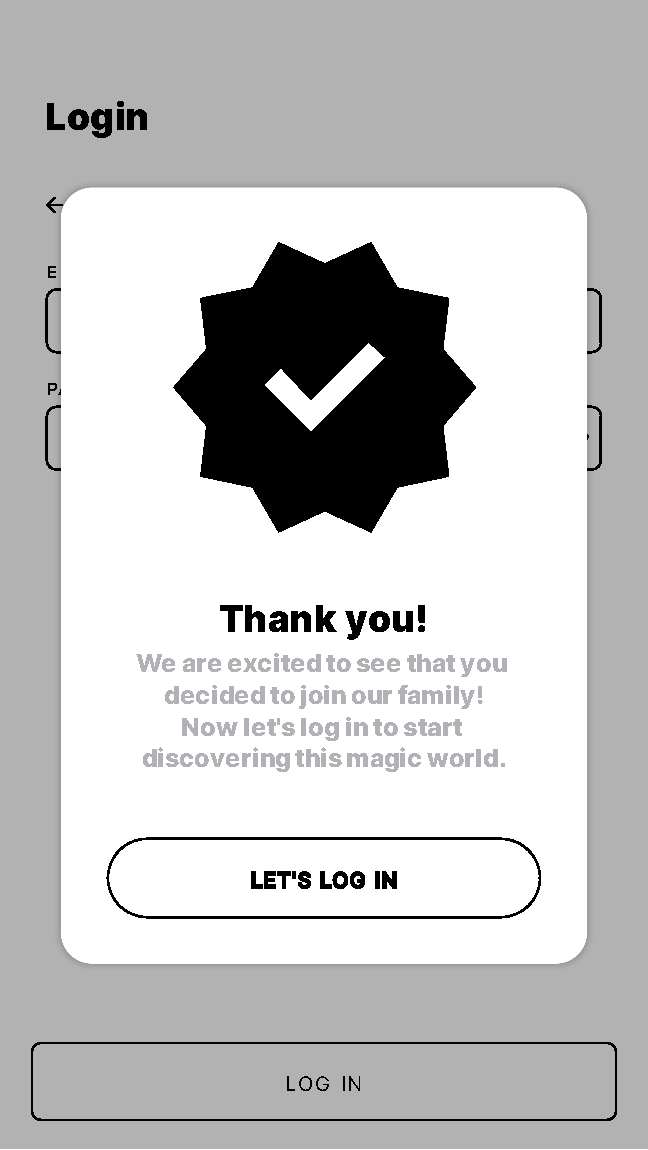
\includegraphics[width=\textwidth]{images/mockups/emsp/signup_login/confirmed}}
        \caption{successful registration message.}
    \end{minipage}
    \hfill
    \begin{minipage}{0.49\textwidth}
        \centering
        \fbox{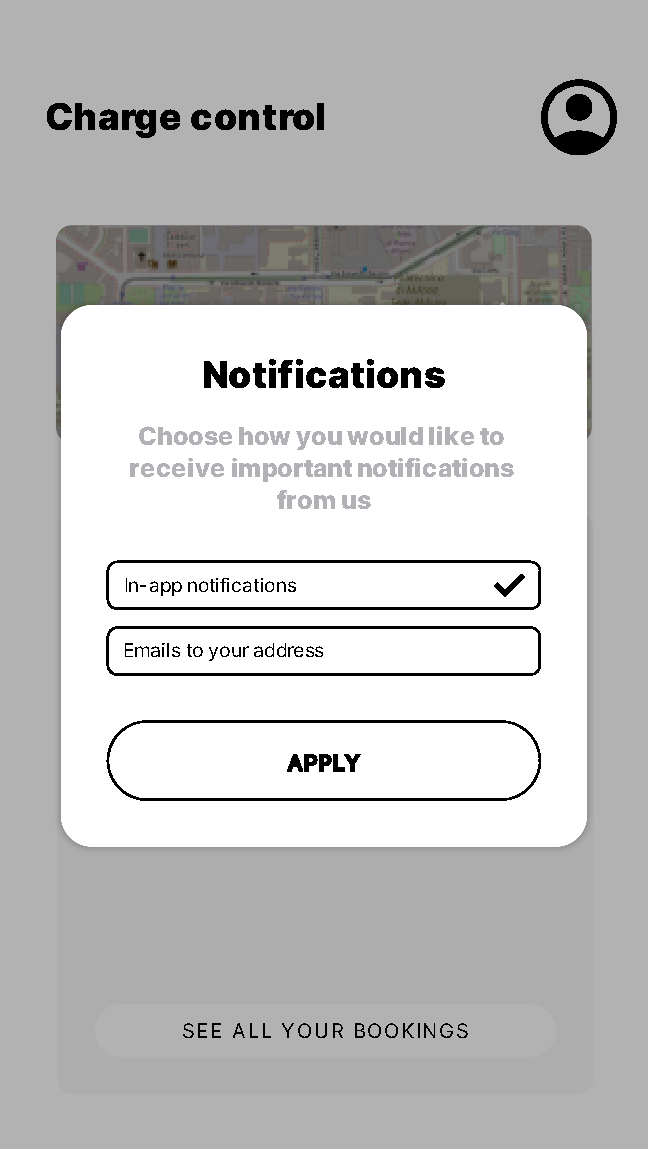
\includegraphics[width=\textwidth]{images/mockups/emsp/signup_login/notification}}
        \caption{first choice of the notification method.}
    \end{minipage}
\end{figure}

\pagebreak

\paragraph{Home page} The home page is the center of the application. From here the user can reach his profile with all the details, the map for booking charges, the history of his charges, and the future ones (which also appear on the home page, as shown in \figureref{figure:ui:emsp:home}), and, if any, a button for paying all the unpaid charges.

\begin{figure}[h!]
    \begin{minipage}{0.49\textwidth}
        \centering
        \fbox{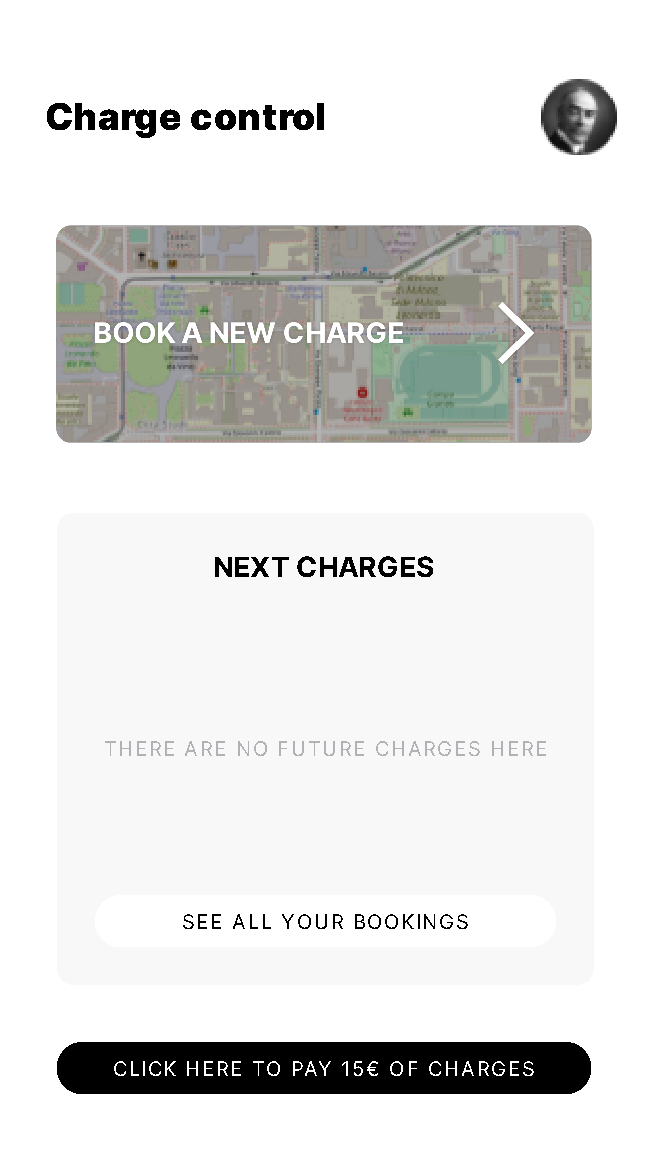
\includegraphics[width=\textwidth]{images/mockups/emsp/homepage_profile/home}}
        \caption{home page with no bookings.}
    \end{minipage}
    \hfill
    \begin{minipage}{0.49\textwidth}
        \centering
        \fbox{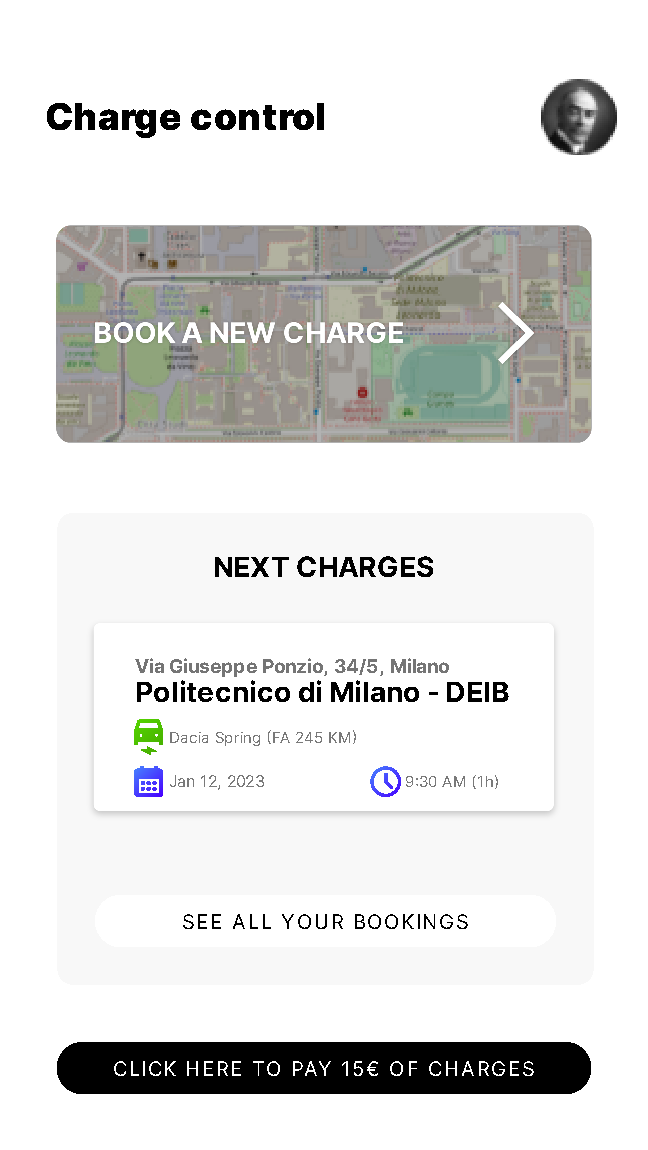
\includegraphics[width=\textwidth]{images/mockups/emsp/homepage_profile/charges}}
        \caption{home page with bookings.}
        \label{figure:ui:emsp:home}
    \end{minipage}
\end{figure}

\pagebreak

\paragraph{User's profile} From this page, the user can see all the data s/he uploaded to the system and can update, download, and delete it. Moreover, from this point, the user can log out from the system, change the preferred notification method and reach his/her vehicles page.

\begin{figure}[h!]
    \begin{minipage}{0.49\textwidth}
        \centering
        \fbox{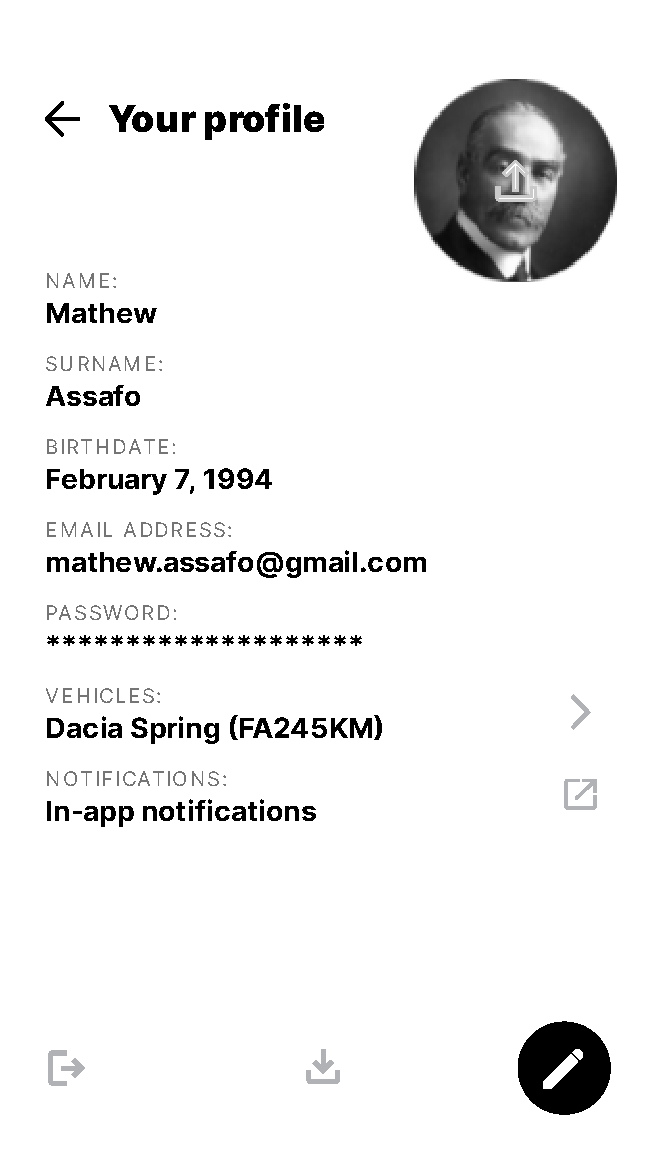
\includegraphics[width=0.71\textwidth]{images/mockups/emsp/homepage_profile/profile}}
        \caption{profile page with all the details.}
    \end{minipage}
    \hfill
    \begin{minipage}{0.49\textwidth}
        \centering
        \fbox{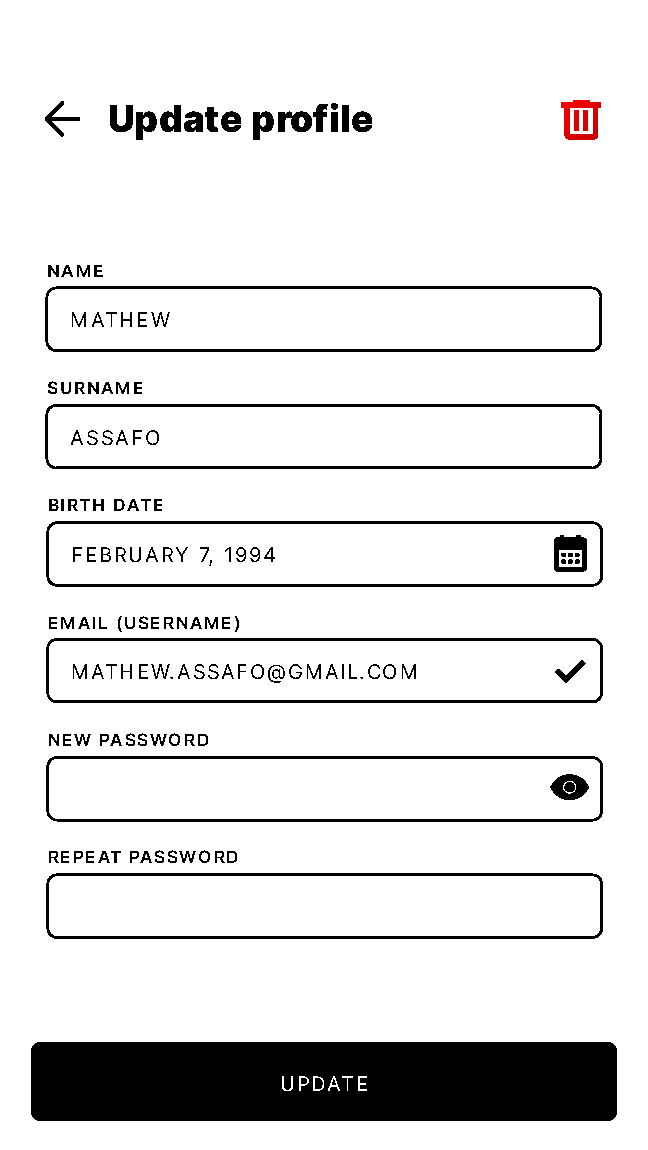
\includegraphics[width=0.71\textwidth]{images/mockups/emsp/homepage_profile/update}}
        \caption{page for profile update.}
    \end{minipage}
\end{figure}
\begin{figure}[h!]
    \centering
    \begin{minipage}{0.49\textwidth}
        \centering
        \fbox{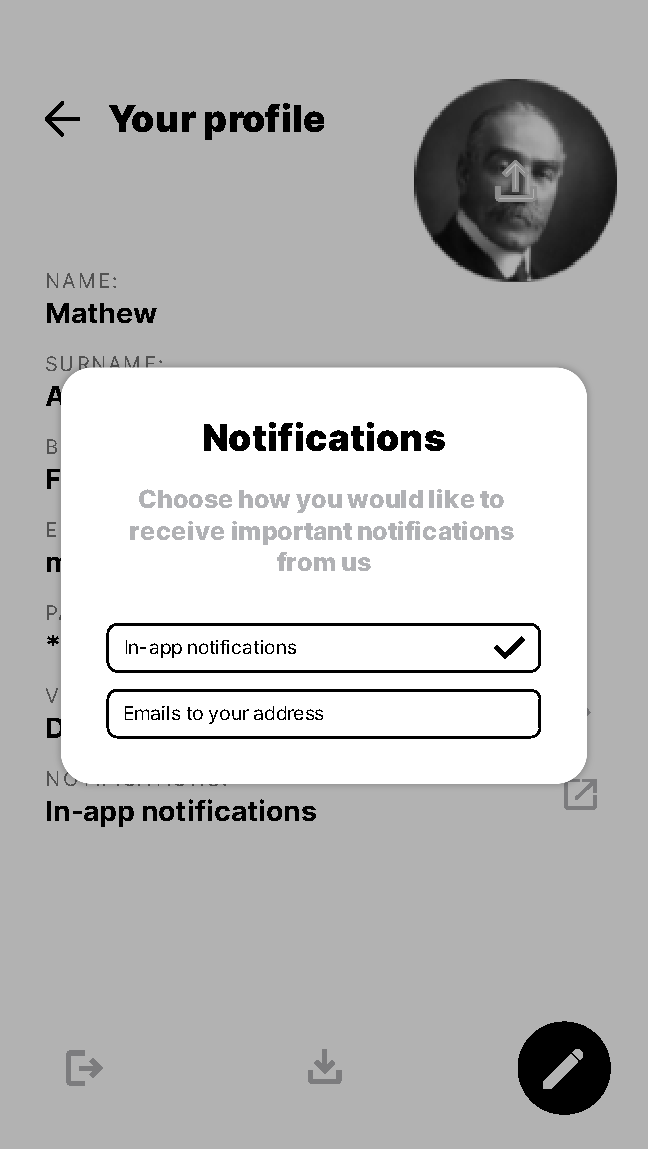
\includegraphics[width=0.71\textwidth]{images/mockups/emsp/homepage_profile/notification}}
    \end{minipage}
    \caption{notification preference change on user's profile.}
\end{figure}

\pagebreak

\paragraph{Stations lookup: map view} The map view allows the user to see all the charging stations around thanks to the use of OpenStreetMap. The user can activate and deactivate the localization functionality, search for a specific location, look at his/her list of favorite stations or move to the list view.

\begin{figure}[h!]
    \begin{minipage}{0.49\textwidth}
        \centering
        \fbox{
\includegraphics[width=\textwidth]{images/mockups/emsp/lookup/map}}
        \caption{map view.}
    \end{minipage}
    \hfill
    \begin{minipage}{0.49\textwidth}
        \centering
        \fbox{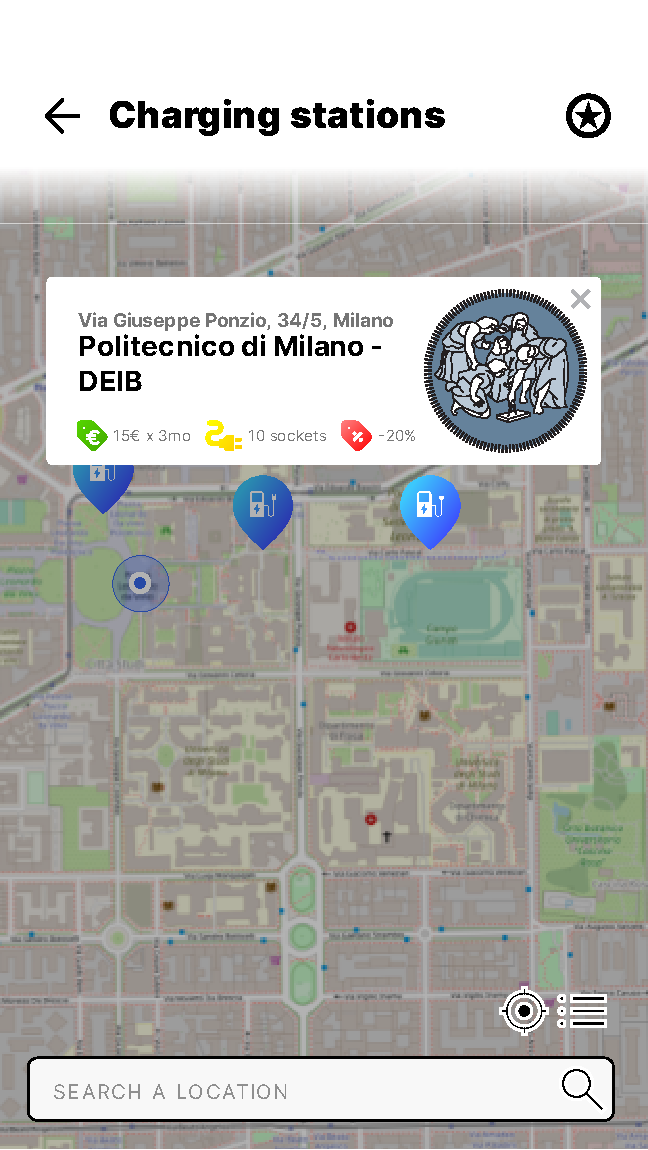
\includegraphics[width=\textwidth]{images/mockups/emsp/lookup/station}}
        \caption{map view when a station is selected.}
    \end{minipage}
\end{figure}

\pagebreak

\paragraph{Stations lookup: list view and favorites} The list view acts like the map view, but instead of presenting the charging stations in the map, it shows them in a list form which allows the user to sort them according to various parameters\footnote{The popup used for selecting the sorting parameters is the classical one of each system, so it's not represented here, but it includes the distance from the selected point, the price (with the presence of any eventual discount) and the availability, both in ascending and descending order.}, to go back to the map view or to see the list of favorite stations. Moreover, it allows the user to mark or unmark any station as favorite.

\begin{figure}[h!]
    \begin{minipage}{0.49\textwidth}
        \centering
        \fbox{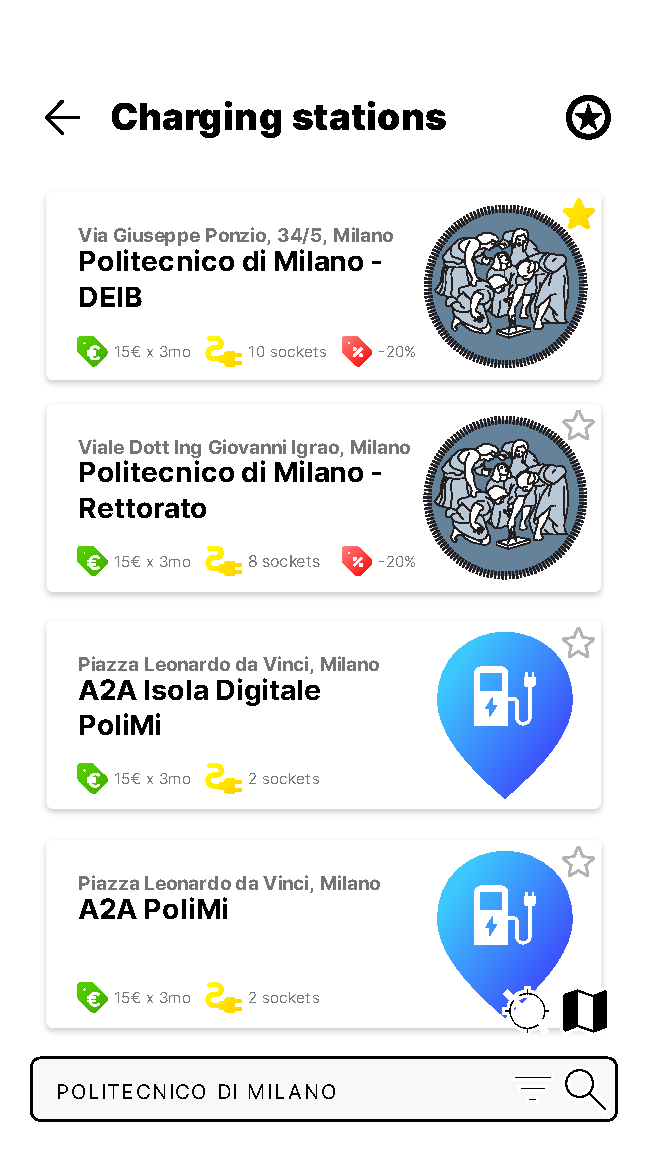
\includegraphics[width=\textwidth]{images/mockups/emsp/lookup/list}}
        \caption{list view.}
    \end{minipage}
    \hfill
    \begin{minipage}{0.49\textwidth}
        \centering
        \fbox{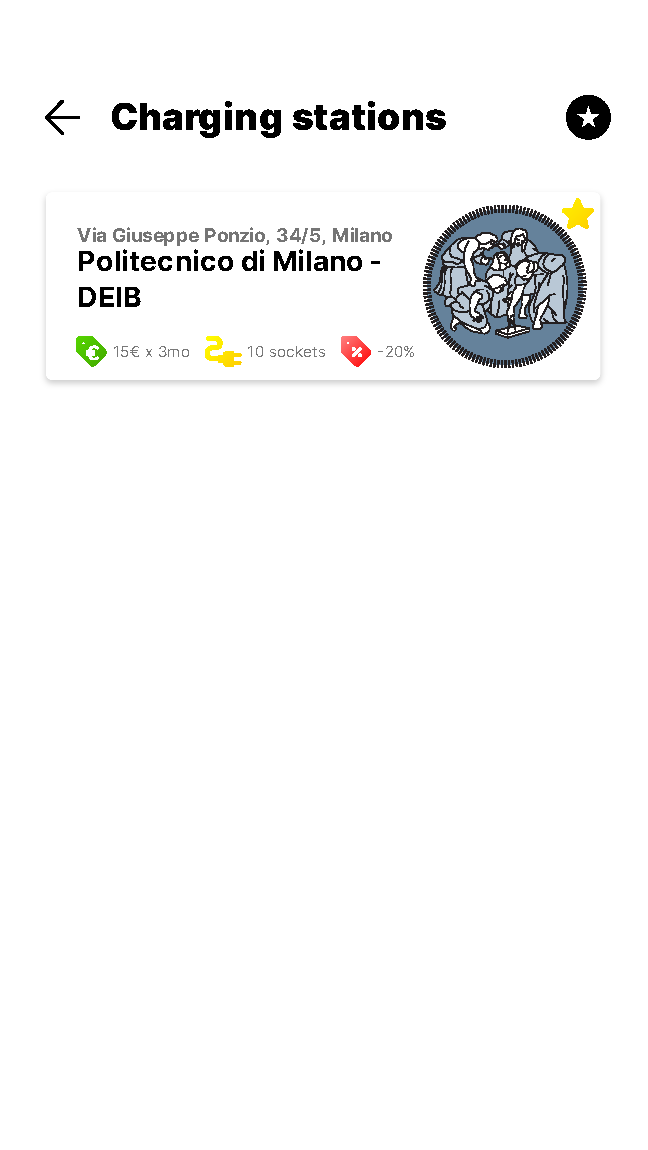
\includegraphics[width=\textwidth]{images/mockups/emsp/lookup/favorites}}
        \caption{favorites view.}
    \end{minipage}
\end{figure}

\vfill

\pagebreak

\paragraph{Book a charge} Once the user has selected from the map or list view a station, s/he can open its page from which he can see all the data of that station and can book a charge (and also can toggle the \doublequotes{favorite} state). Once the user clicks on the booking button, a popup appears giving the possibility to book a slot for a specific date and time for one of his/her vehicles.

\begin{figure}[h!]
    \begin{minipage}{0.49\textwidth}
        \centering
        \fbox{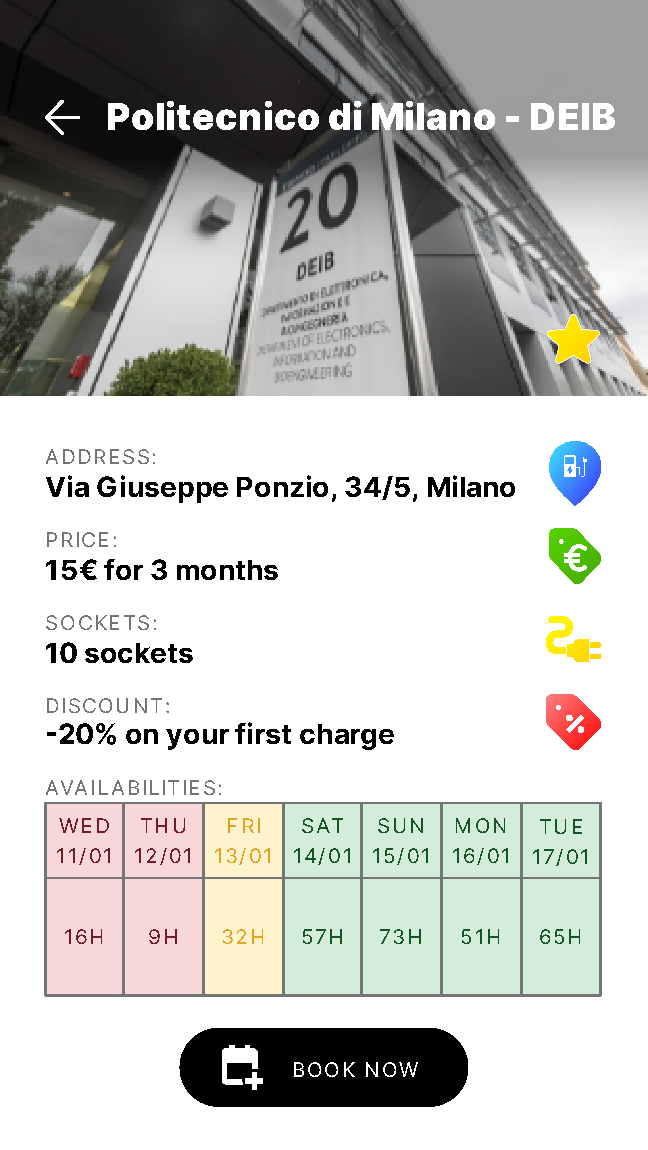
\includegraphics[width=\textwidth]{images/mockups/emsp/booking/station}}
        \caption{charging station's page.}
    \end{minipage}
    \hfill
    \begin{minipage}{0.49\textwidth}
        \centering
        \fbox{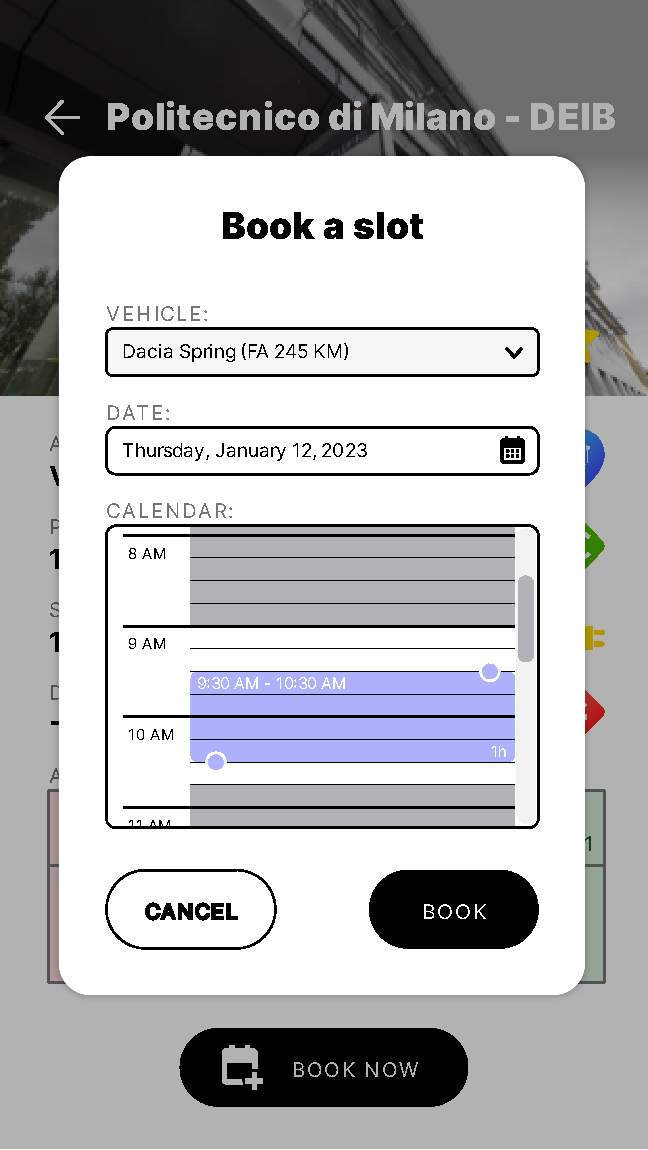
\includegraphics[width=\textwidth]{images/mockups/emsp/booking/booking}}
        \caption{station's page with booking popup.}
    \end{minipage}
\end{figure}

\pagebreak

\paragraph{Bookings views} This view can be reached from the home page and lists all the future and past bookings of the user. Any future (or current) charge can be opened on a dedicated page in order to show all the details (including the assigned slot if present) and can be edited or deleted. Moreover, the red past bookings are the ones that still have to be paid, and for doing that there is an apposite button on the end of the page.

\begin{figure}[h!]
    \begin{minipage}{0.49\textwidth}
        \centering
        \fbox{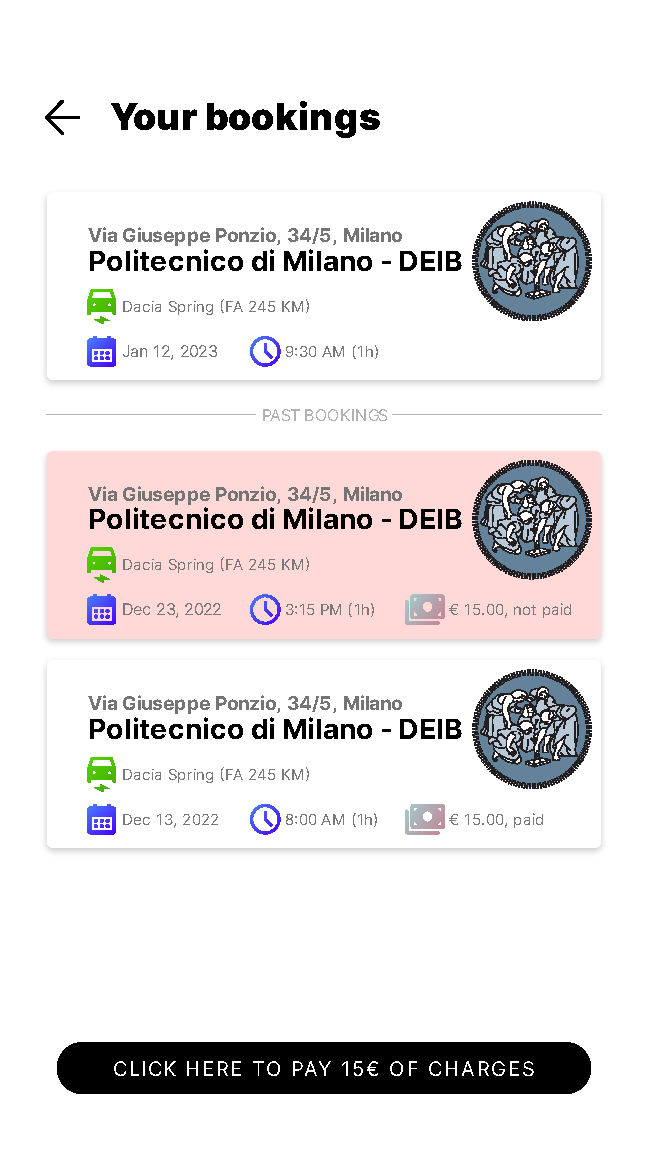
\includegraphics[width=0.71\textwidth]{images/mockups/emsp/bookings/bookings}}
        \caption{the page with all the bookings.}
    \end{minipage}
    \hfill
    \begin{minipage}{0.49\textwidth}
        \centering
        \fbox{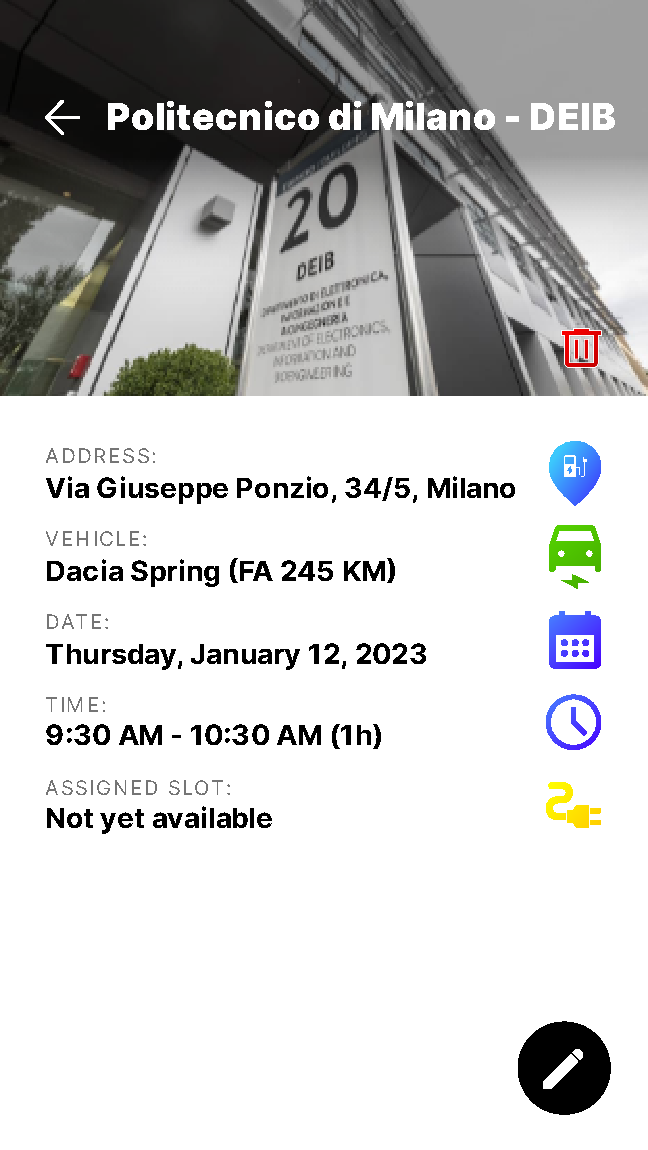
\includegraphics[width=0.71\textwidth]{images/mockups/emsp/bookings/details}}
        \caption{a booking page with all the details.}
    \end{minipage}
\end{figure}
\begin{figure}[h!]
    \centering
    \begin{minipage}{0.49\textwidth}
        \centering
        \fbox{
\includegraphics[width=0.71\textwidth]{images/mockups/emsp/bookings/edit}}
    \end{minipage}
    \caption{the editing popup of the booking.}
\end{figure}

\pagebreak

\paragraph{Vehicles} The user can add a new vehicle, update it or delete it at any time. If the change interests some future charge (in general, any non-started charge), the system acts as a consequence as stated in chapter \reference{architecture}, for example deleting the booking or updating the certificate for the charge.

\begin{figure}[h!]
    \begin{minipage}{0.49\textwidth}
        \centering
        \fbox{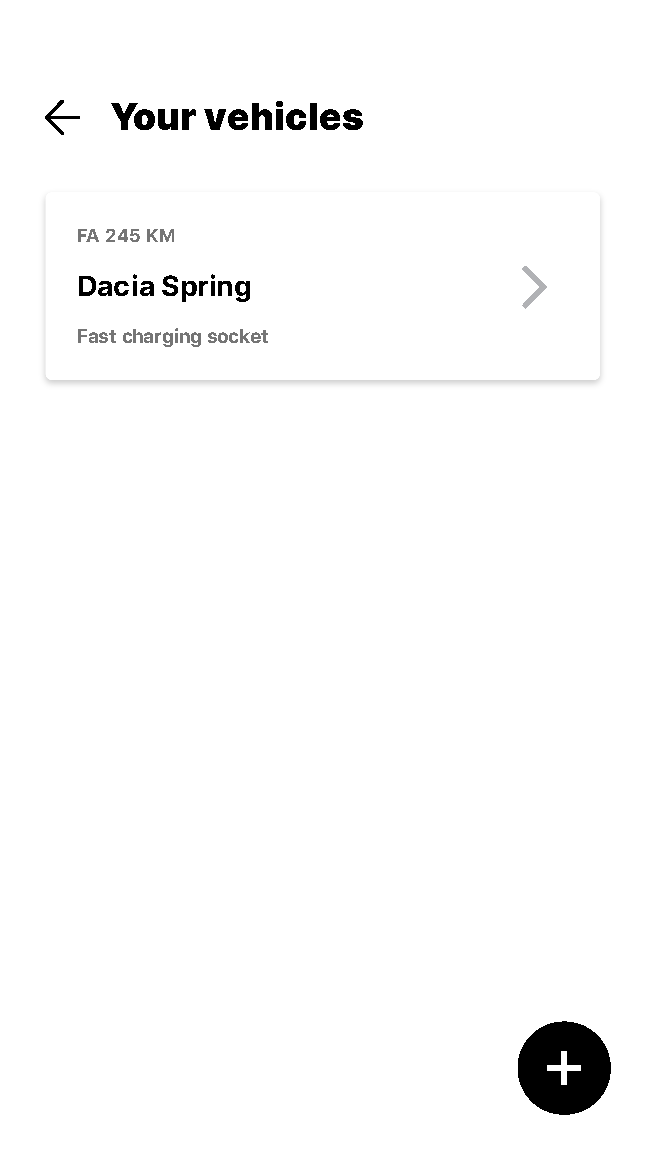
\includegraphics[width=0.71\textwidth]{images/mockups/emsp/vehicles/vehicles}}
        \caption{the page with all the vehicles.}
    \end{minipage}
    \hfill
    \begin{minipage}{0.49\textwidth}
        \centering
        \fbox{
\includegraphics[width=0.71\textwidth]{images/mockups/emsp/vehicles/add}}
        \caption{the popup for adding a new vehicle.}
    \end{minipage}
\end{figure}
\begin{figure}[h!]
    \begin{minipage}{0.49\textwidth}
        \centering
        \fbox{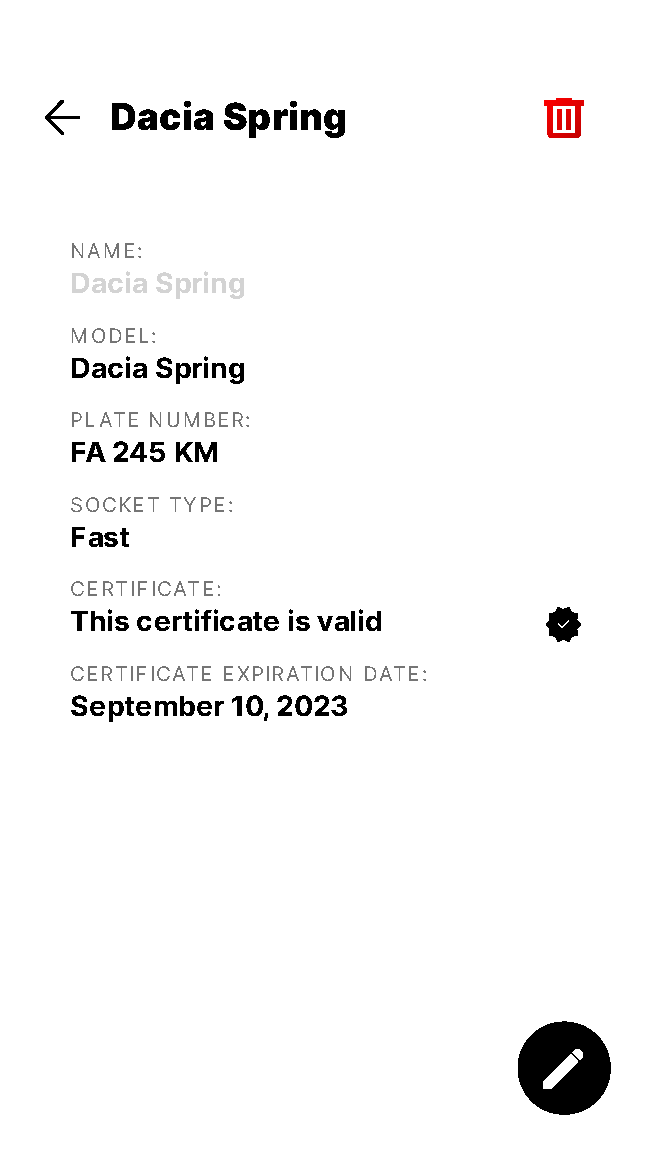
\includegraphics[width=0.71\textwidth]{images/mockups/emsp/vehicles/vehicle}}
        \caption{the details of a vehicle.}
    \end{minipage}
    \hfill
    \begin{minipage}{0.49\textwidth}
        \centering
        \fbox{
\includegraphics[width=0.71\textwidth]{images/mockups/emsp/vehicles/edit}}
        \caption{the popup for editing a vehicle.}
    \end{minipage}
\end{figure}

\pagebreak

\paragraph{Payment} Before the user pays from the application the charges, the system shows this page allowing him/her to choose the method s/he prefers for paying. The system supports multiple transaction managers like the ones shown in this interface, but it can be expanded in the future to support more.

\begin{figure}[h!]
    \centering
    \fbox{
\includegraphics[width=0.49\textwidth]{images/mockups/emsp/payment}}
    \caption{the choice of the payment method.}
\end{figure}

\pagebreak

\subsection{Pages connections}

This diagram shows how all the presented interfaces are connected. The white circle at the top left of the diagram presents the starting point, which can be either the opening of the application or the opening of the private area on the eMSP's website.

\begin{figure}[h!]
    \centering
    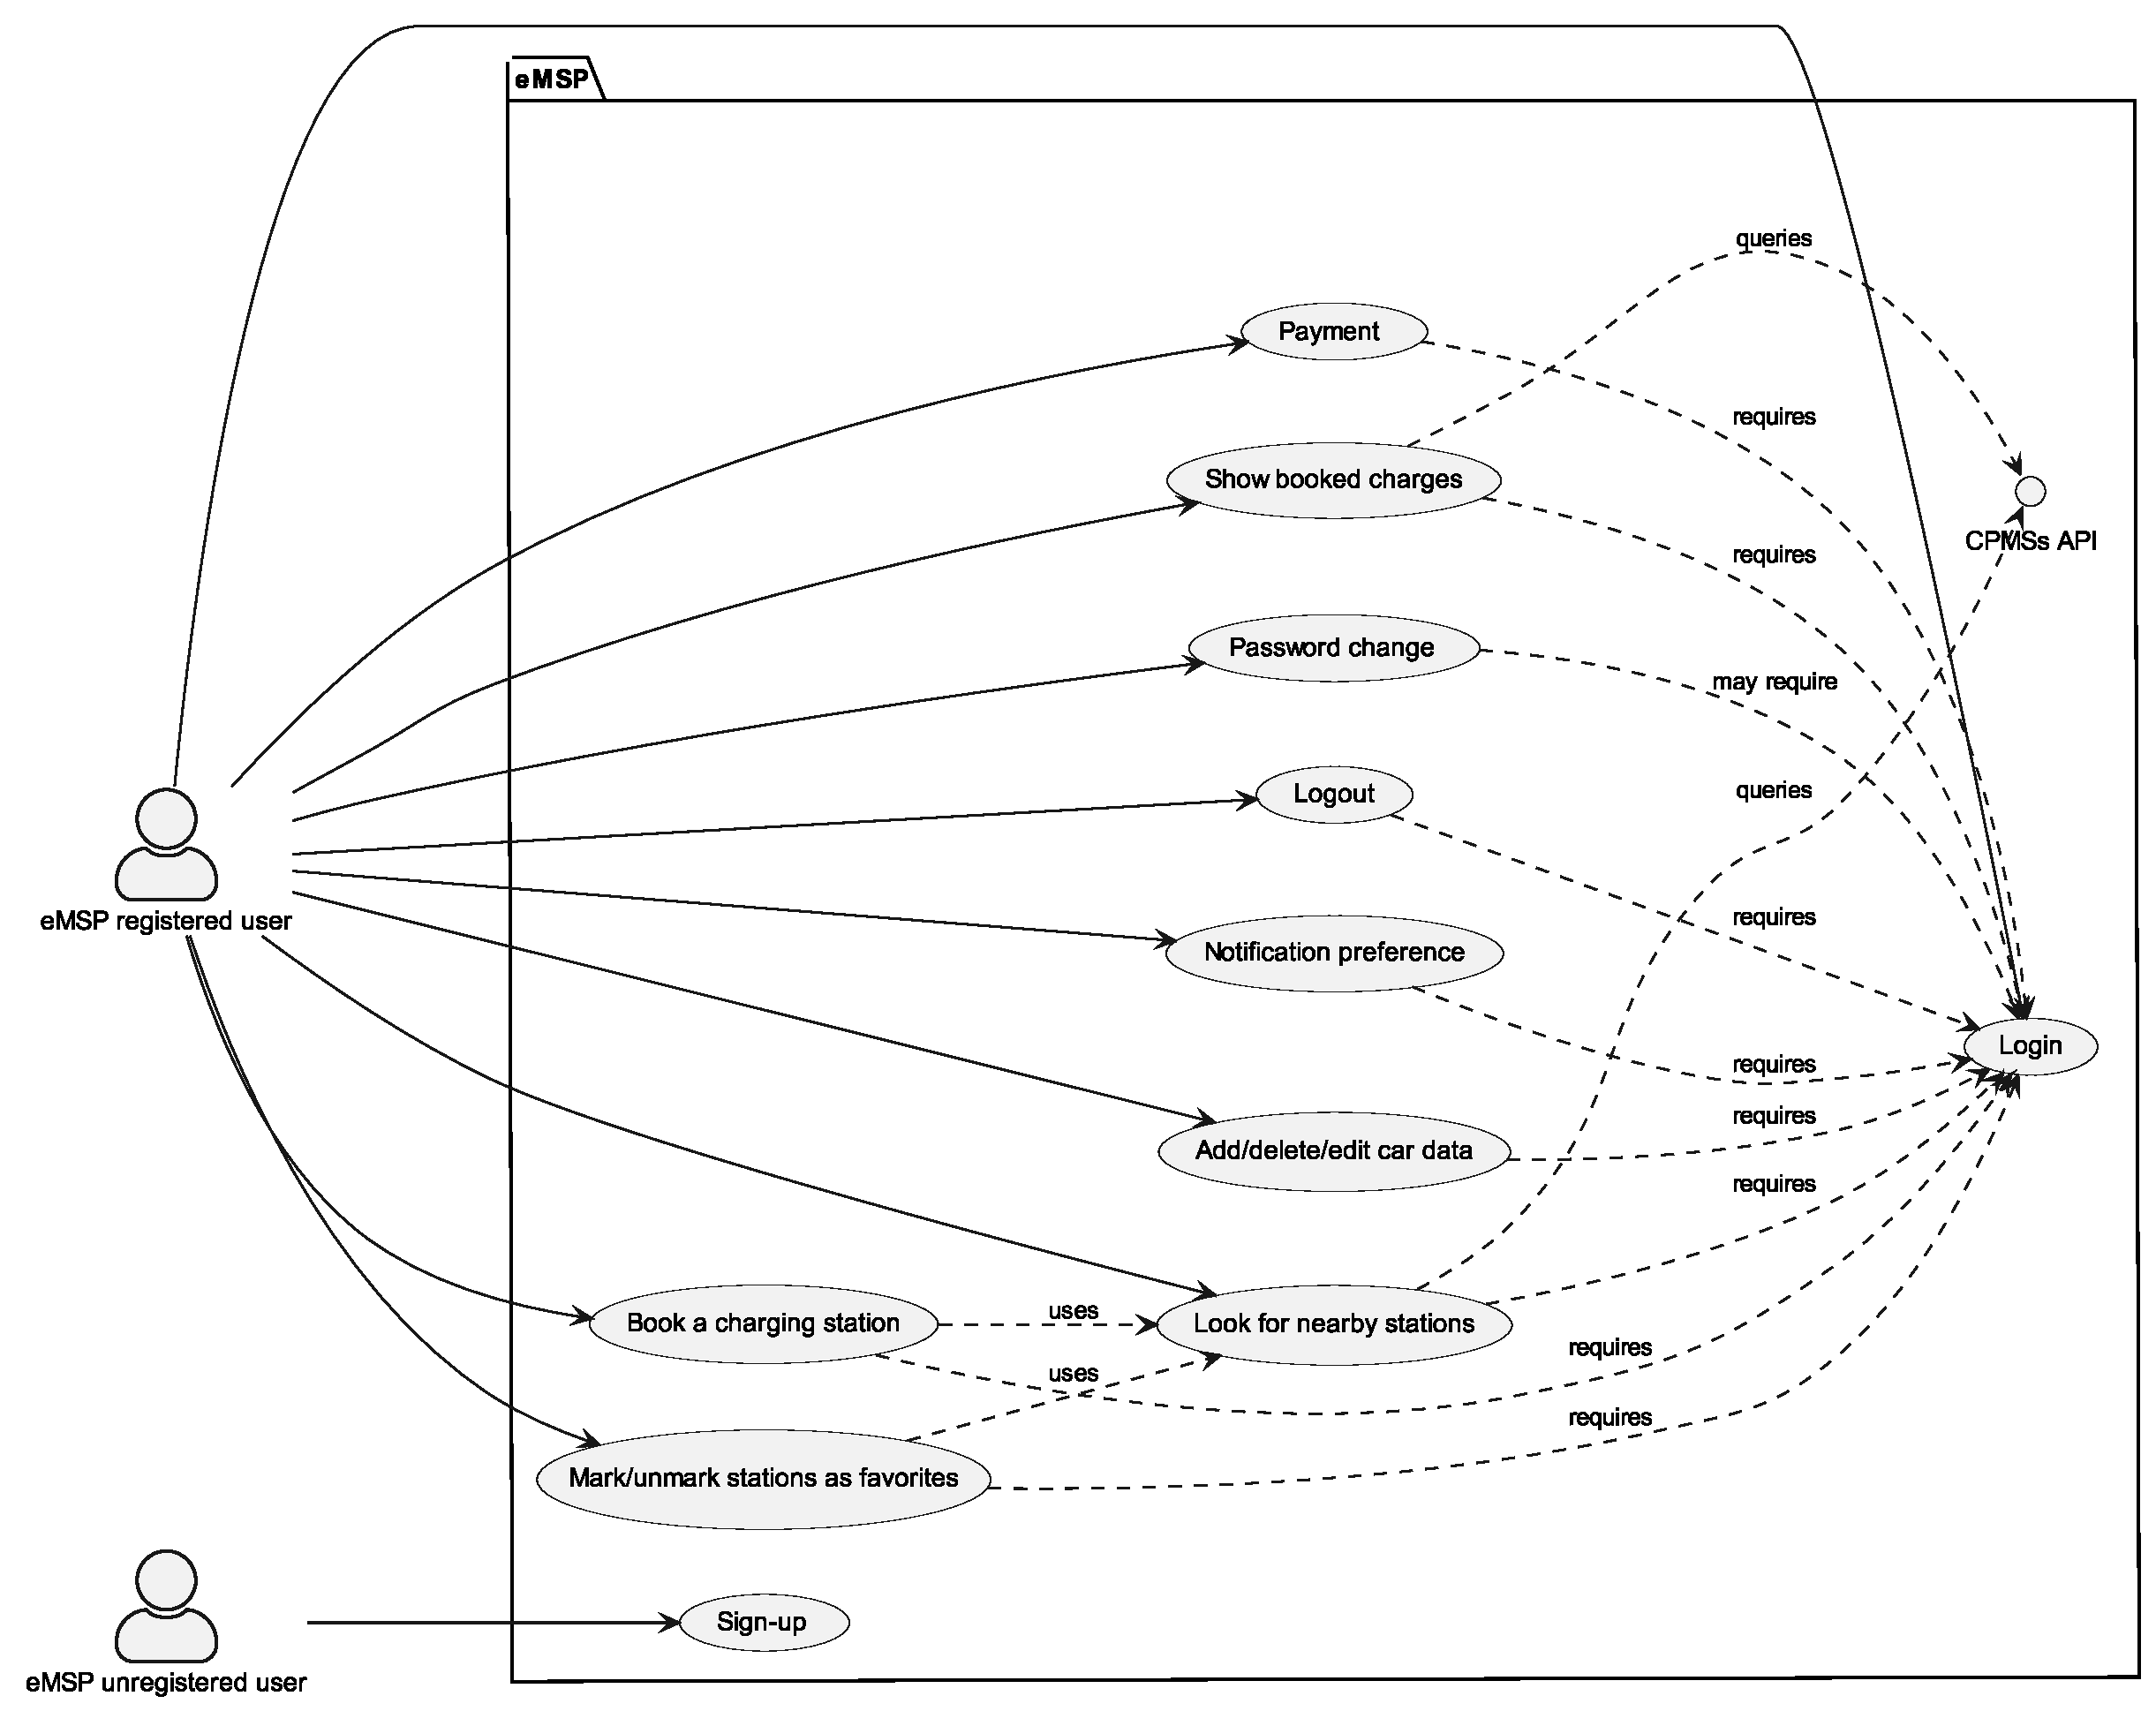
\includegraphics[width=\columnwidth]{./images/connections/emsp}
    \caption{the connections between the various interfaces.}
\end{figure}

\section{CPMS}

Interactions with the CPMS system are conducted by authorized CPMS users. These users are expected to interact with the CPMS to carry out occasional tasks, as the main system is thought to be automatized. Nonetheless, the CPMS system offers a website capable of allowing all reasonable actions to the users, with an immediate and fairly easy-to-use interface. In this section, mockups of the website are presented to resemble what the actual site could look like. 

\subsection{Interfaces design}

To represent the website for the CPMS system, instances of a \textit{Firefox} browser from a \textit{macOS}-looking operating system are shown, but any browser on any operating system would work, as long as it's running on a working computer. Viewing the website from a mobile phone would be strongly discouraged. 

\paragraph{Login} In order to access the website, users must first login through the login page. The standard username and password are the only requirements, but the system can be expanded to include the need for a second factor for authentication.

\bigskip
\bigskip
\bigskip
\bigskip

\begin{figure}[h!]
    \centering
    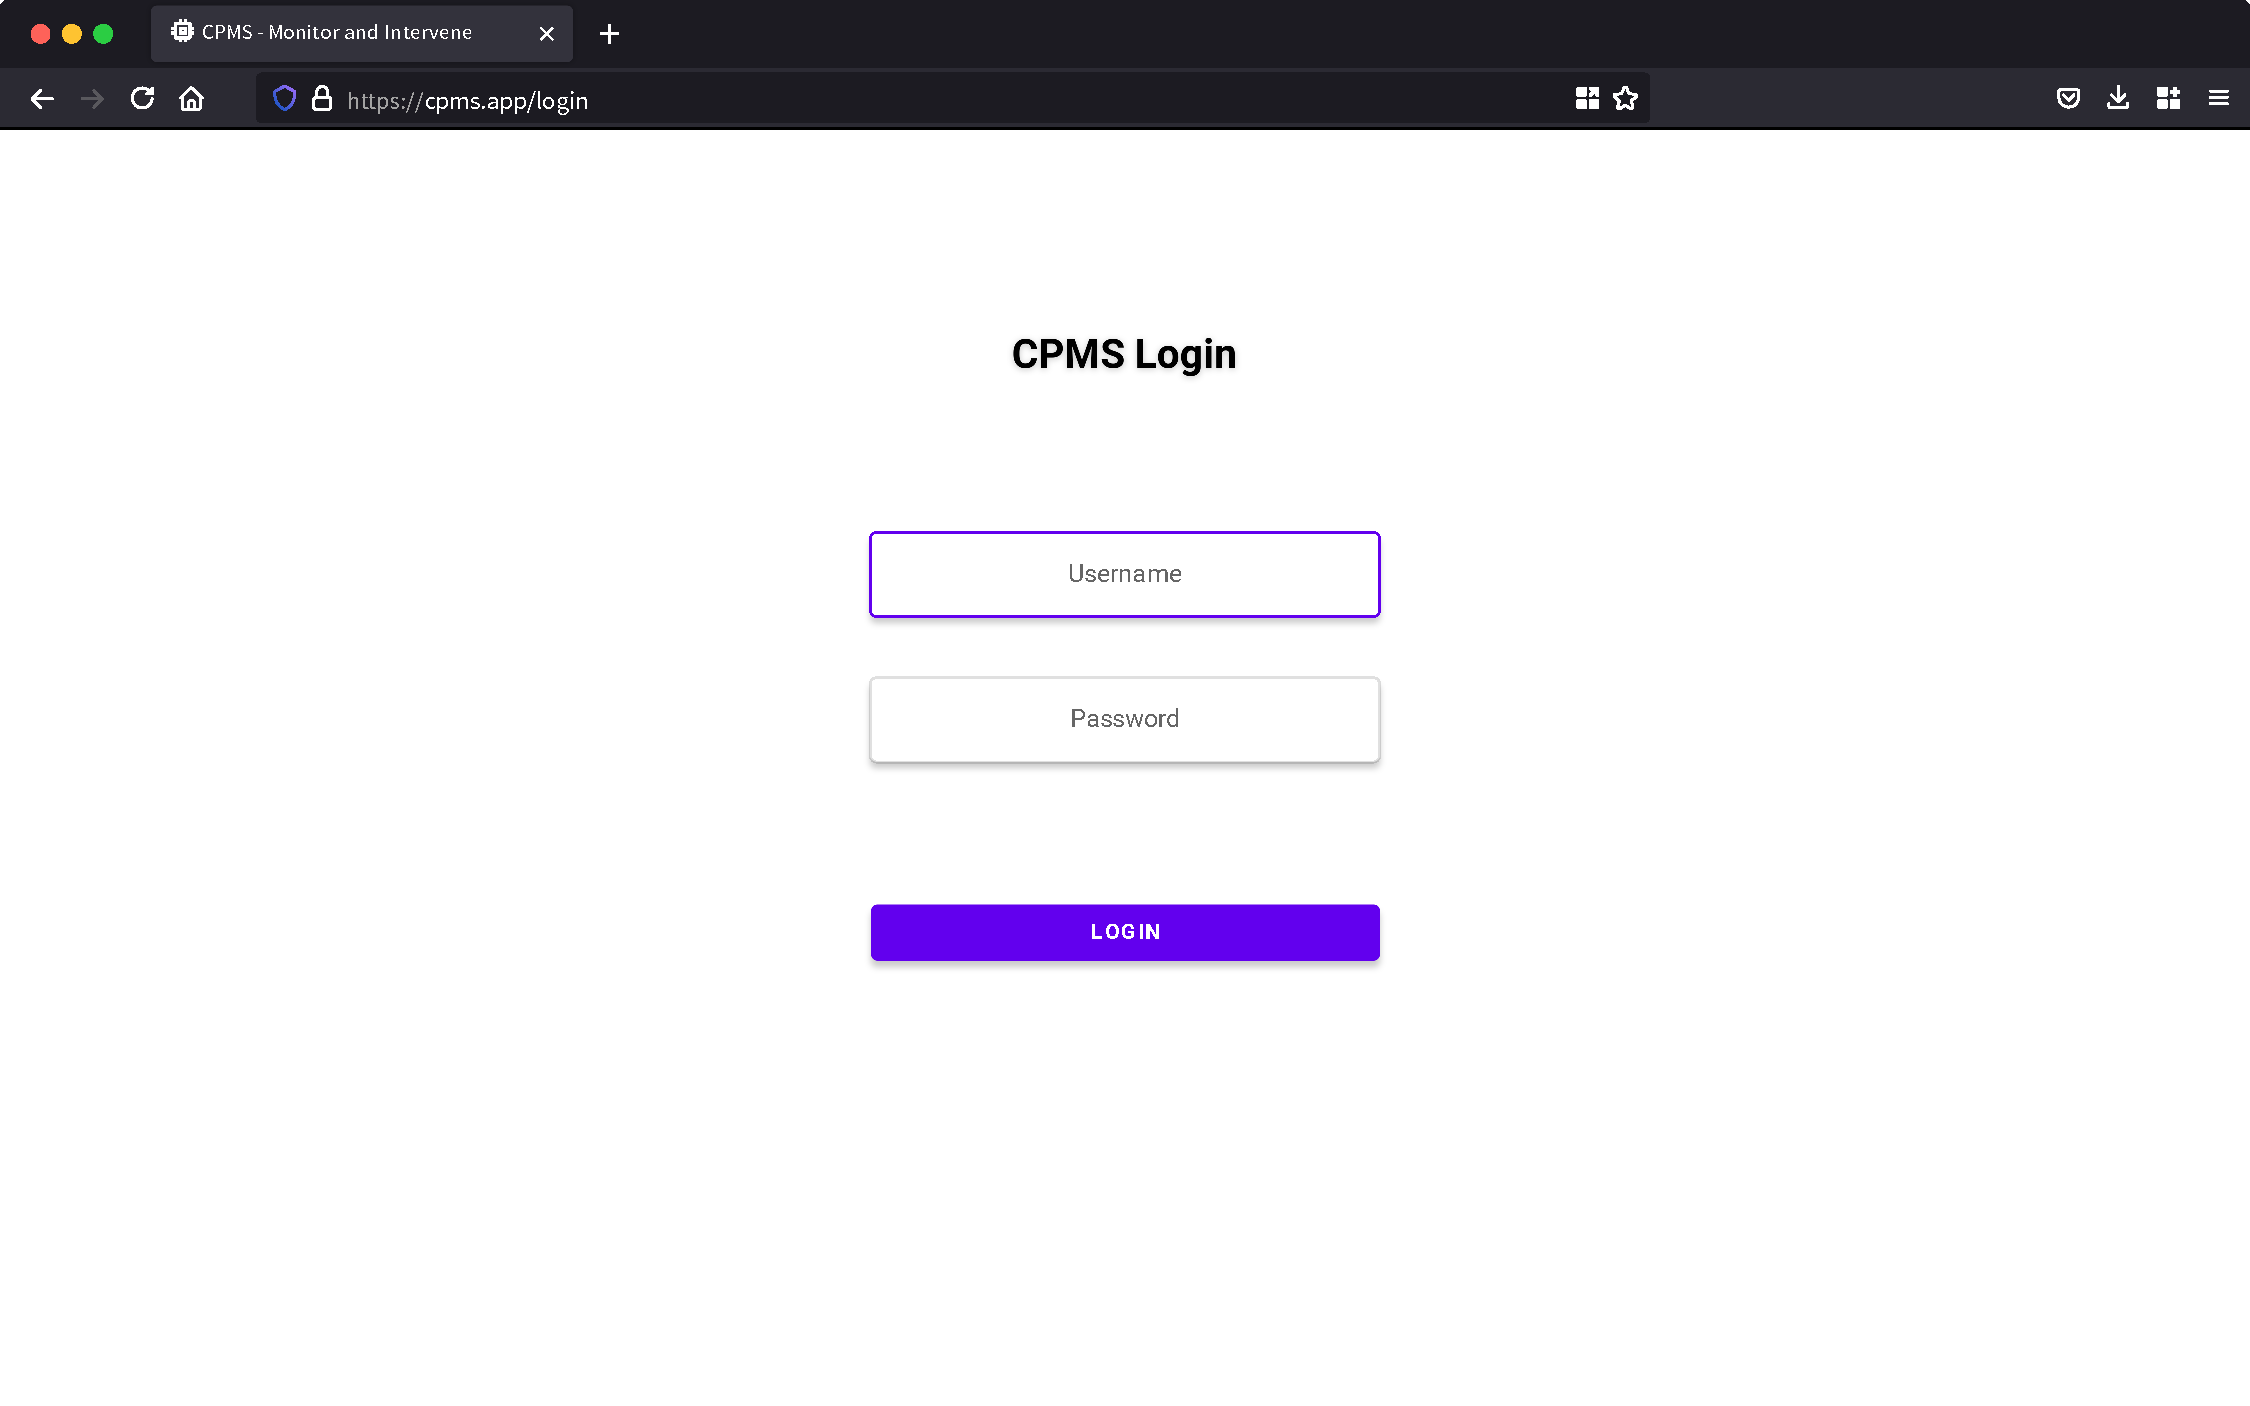
\includegraphics[width=\columnwidth]{./images/mockups/cpms/login}
    \caption{CPMS login page.}
\end{figure}

\pagebreak

\paragraph{Home} After login, the web server sends the user the home page, then sends JSON files containing data on DSOs and stations managed by the user. The home page comprehends a brief statistic tab on a selected station for a selected metric, the central tab needed to access the station page of a selected station, and a brief statistic tab on all DSOs available to any of the stations. A button to go to the special offer page sits underneath the station tab. In the top left corner, a menu tab can be clicked to navigate the site, mainly to return to the home page or to go to the offers page. In the top right corner, the user tab can be clicked to see the user information, to change the password, or to log out of the website. In the bottom left corner, buttons are present to help navigate the website, for general information, and to send emails or to call for support. All the tabs and buttons in the corners are also present on the other pages of the website. 

\bigskip
\bigskip
\bigskip
\bigskip

\begin{figure}[h!]
    \centering
    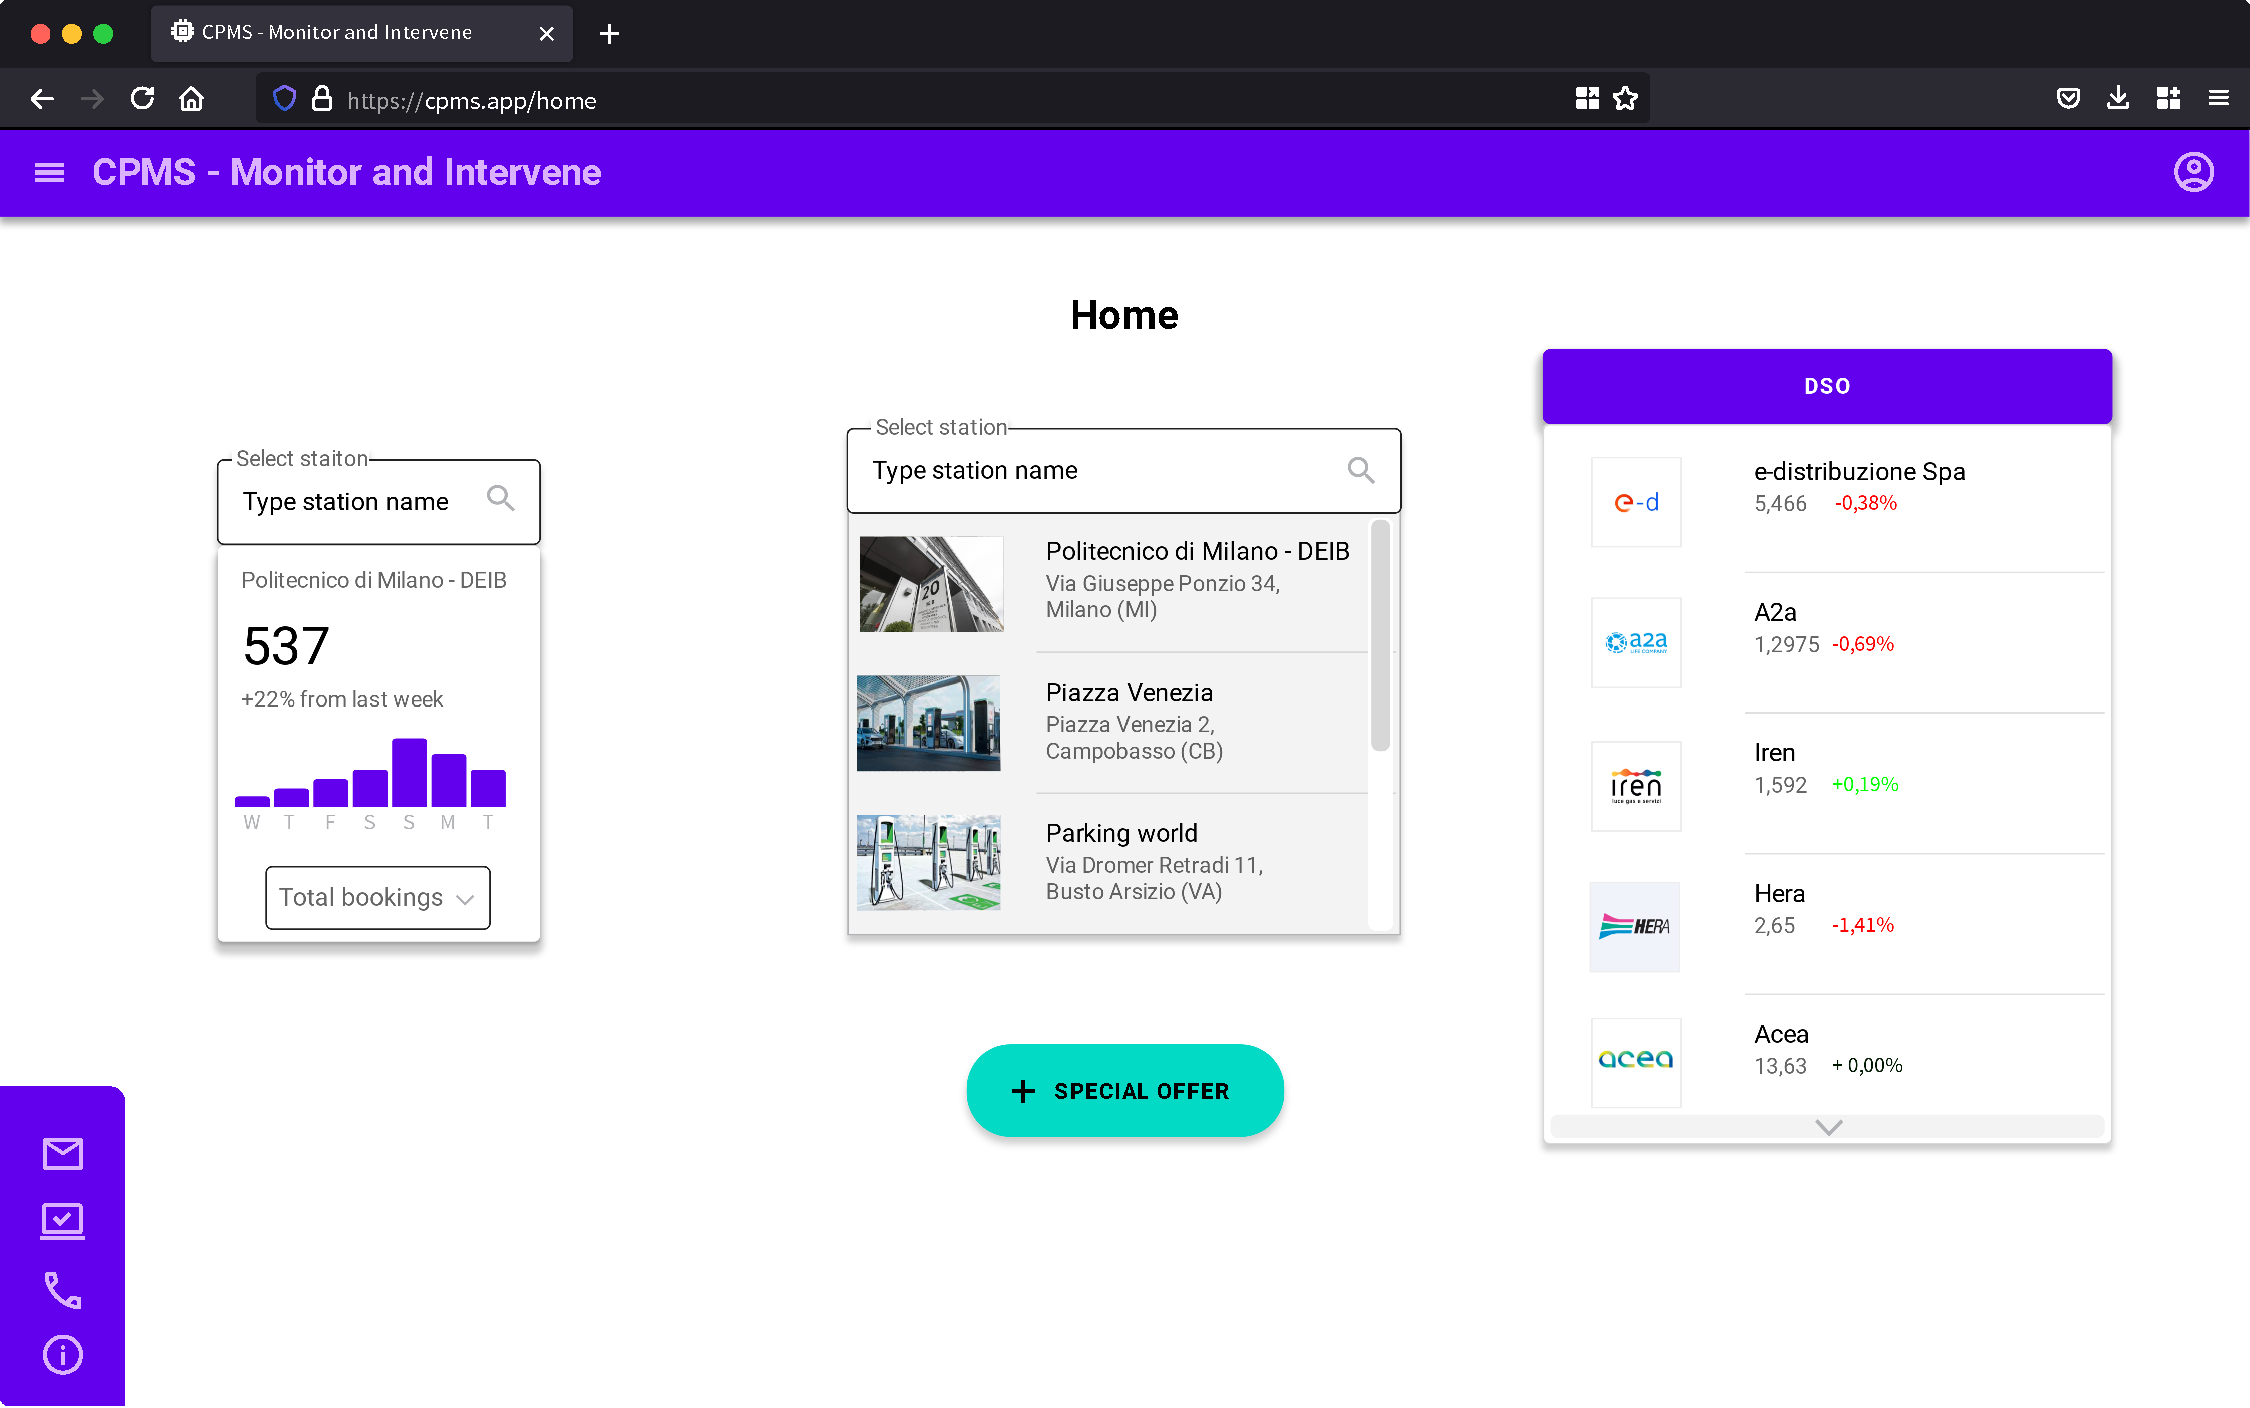
\includegraphics[width=\columnwidth]{./images/mockups/cpms/home}
    \caption{CPMS home page.}
\end{figure}

\pagebreak

\paragraph{Station} By searching (and then clicking on) a charging station, the web server sends the station page, then send data on the sources and DSO available, along with data on the state of the charging columns. On the station page, there are three main tabs. These are periodically updated with new data by the web server. \medskip

The tab in the middle informs the user of the various charging columns present in the charging station, along with information on their socket types and if they are free or occupied at the time of viewing.

\medskip
The left tab is the DSO tab: if the automatic choice is selected (by pressing the button on top), this tab only informs of the DSO available to the station and the prices they offer, along with the currently selected DSO. Otherwise, the user is able to manually and statically select the preferred DSO by clicking on the button on the side of it.
\medskip

The right tab is dedicated to the energy mix. By clicking on the bottom on top the user activates or deactivated the automatic mix choice. If the mix choice is set to manual, users can select if a source can be used or not, and if batteries are present, if these are to be charged or not (batteries cannot be charged while they are in use). The system will still check if illegal states are being reached by the manual choice of an energy mix, and take countermeasures consequently. For example, if not enough power can be obtained by the current setup, and the DSO energy is not being used, the system will automatically set the DSO energy to be used, and will communicate this choice to the user with the next periodic update of the page. Information on the charge level of the batteries and the power obtained from each source is also displayed in this tab.

\bigskip
\bigskip
\bigskip
\bigskip

\begin{figure}[h!]
    \centering
    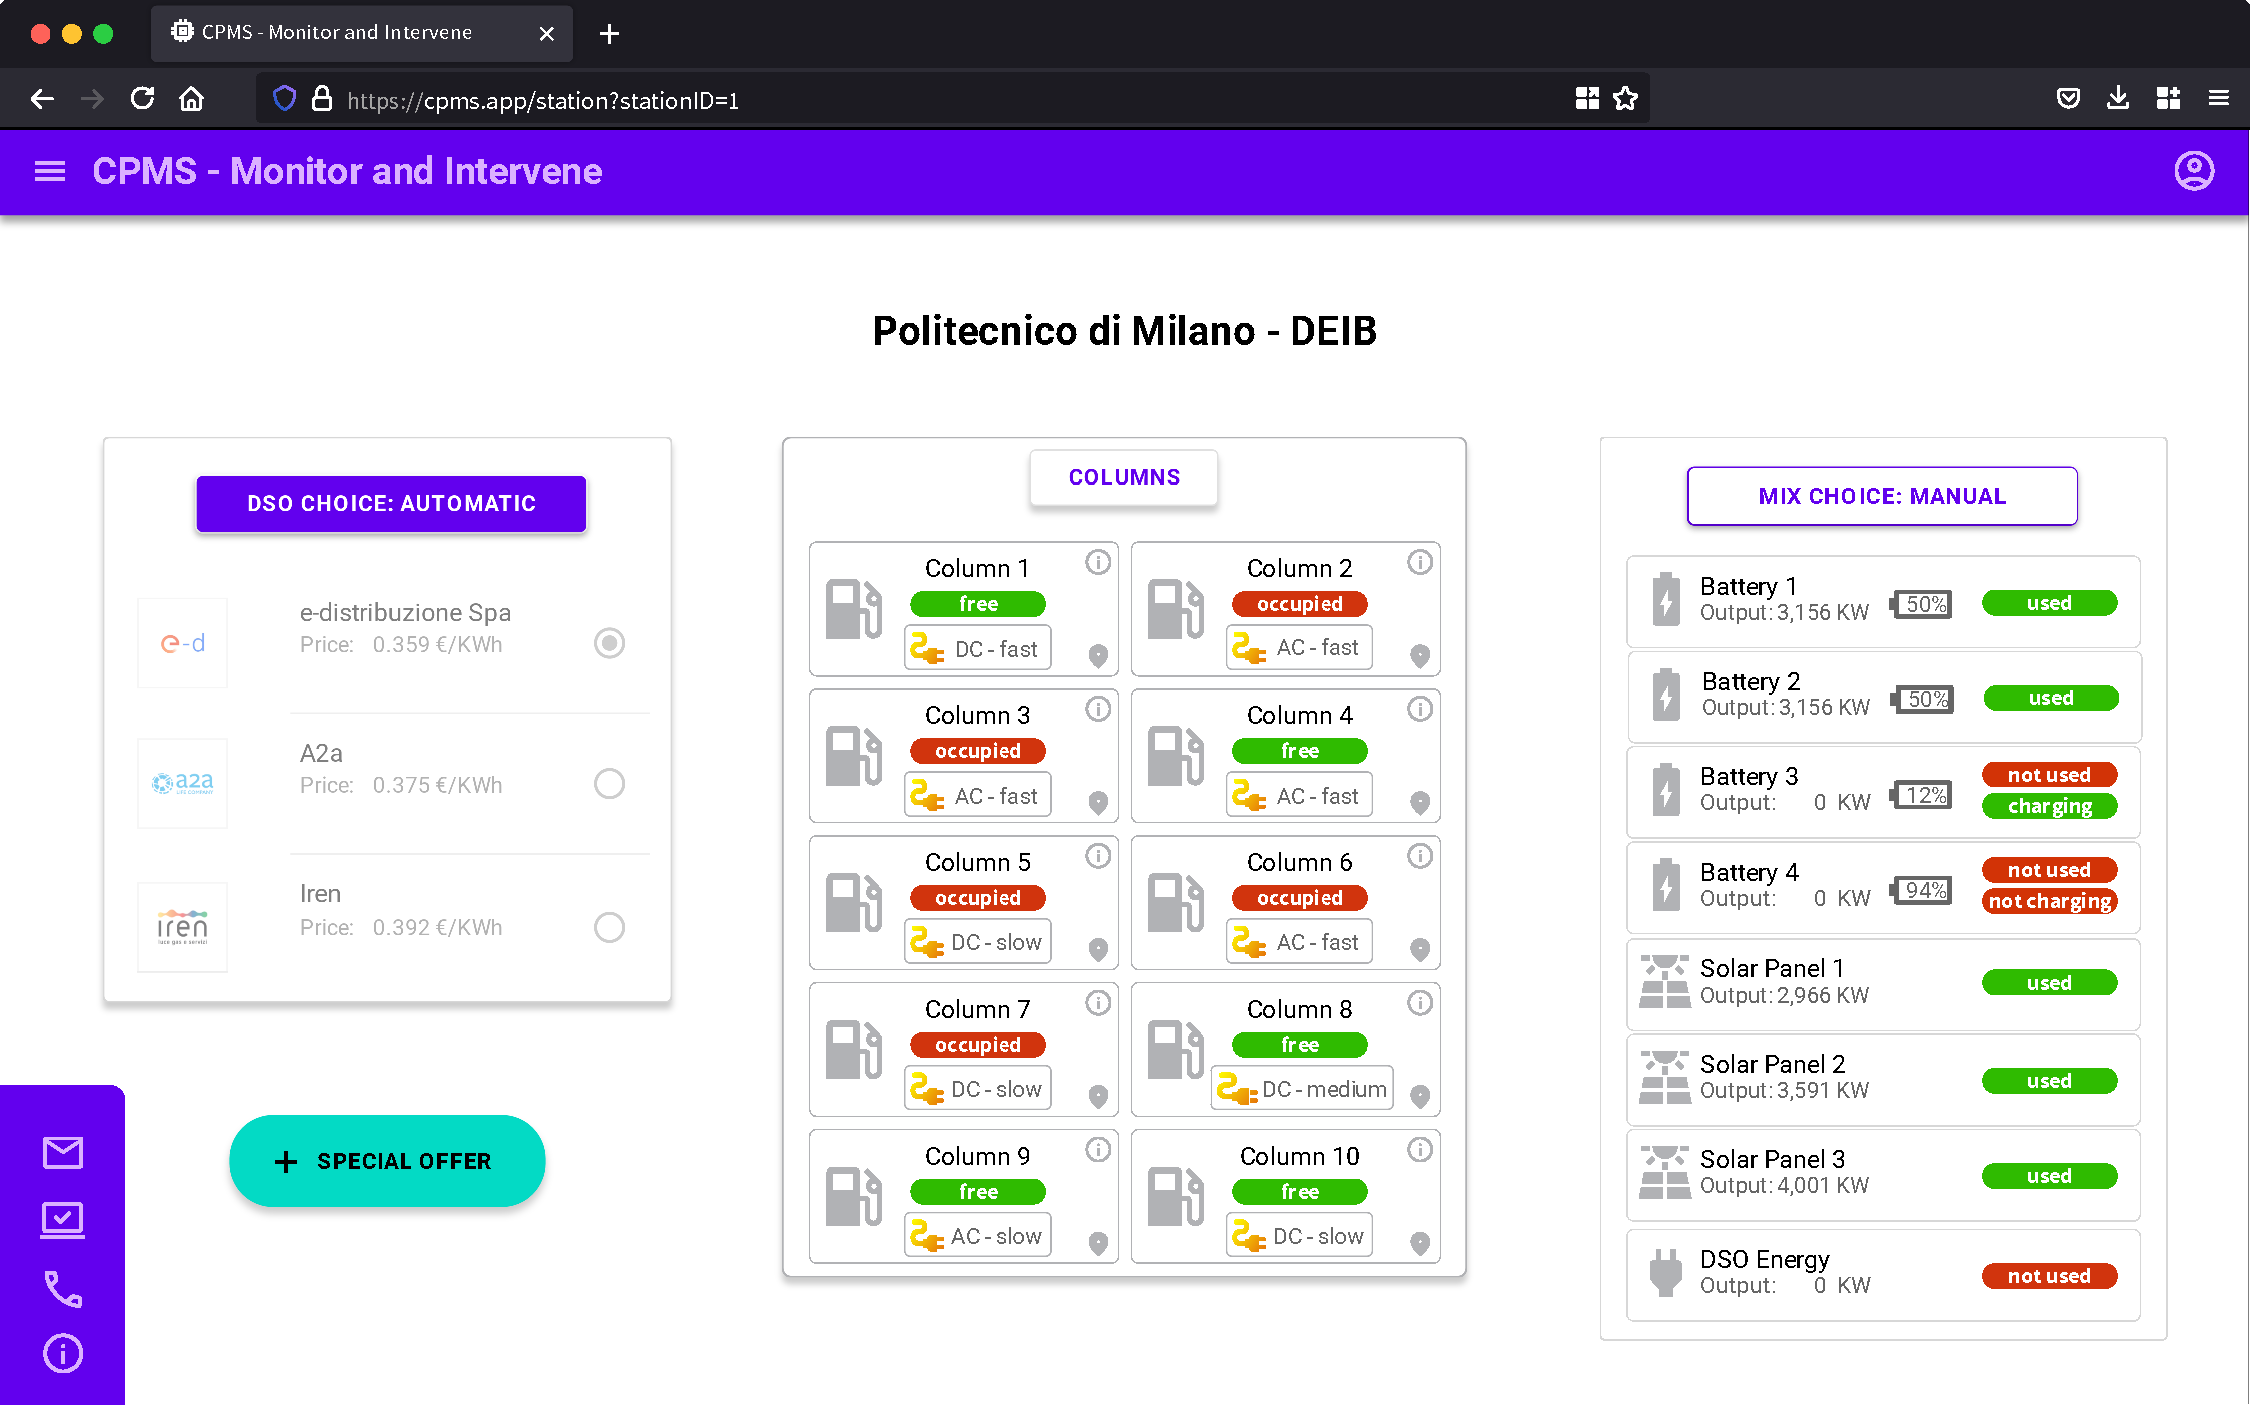
\includegraphics[width=\columnwidth]{./images/mockups/cpms/Station}
    \caption{Charging station page.}
\end{figure}

\pagebreak

\paragraph{Special offer} In the special offer page, users can see all special offers present, and decide if they want to delete them or create a new special offer. A new special offer is created by clicking on the blue button with the plus sign. A pop-up appears where information on the new special offer is asked: the user has to select a start date (from the current day forward), an end date (that comes after the start date), one charging station affected (or all stations if that's the case) and the percentage amount of the discount. By clicking on \doublequotes{Create} the new special offer is created, by clicking on the \doublequotes{x} mark the whole creation is aborted.

\bigskip
\bigskip
\bigskip
\bigskip

\begin{figure}[h!]
    \centering
    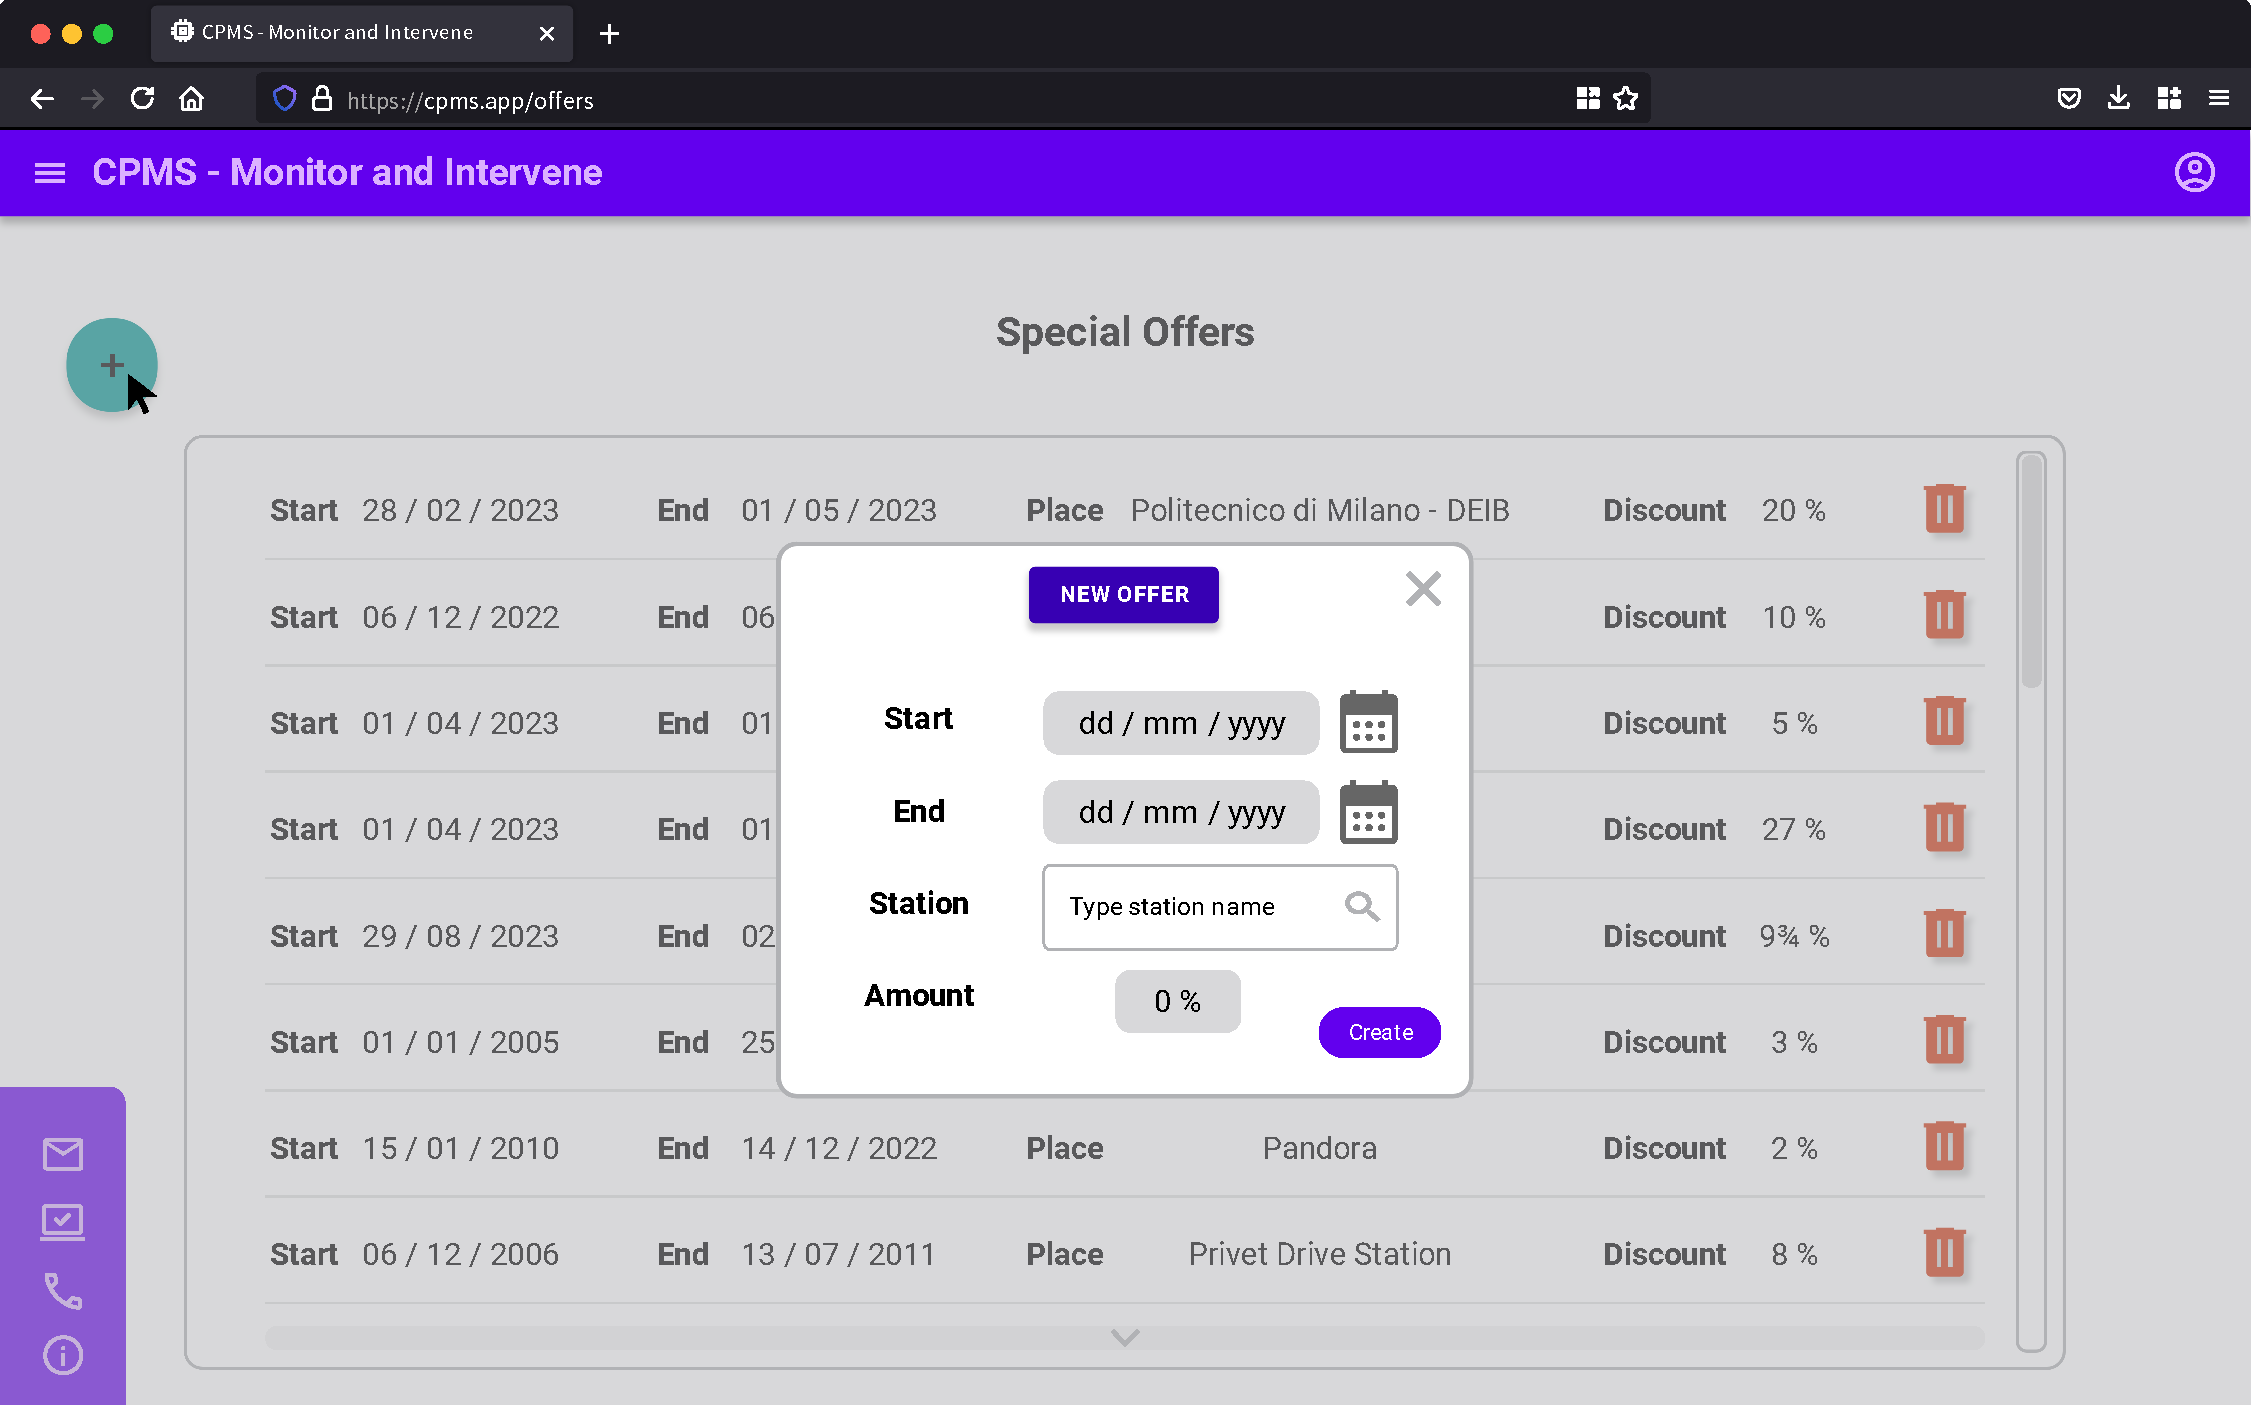
\includegraphics[width=\columnwidth]{./images/mockups/cpms/Offer}
    \caption{Charging station page.}
\end{figure}

\pagebreak

\subsection{Pages connections}

This diagram shows how all the presented interfaces are connected. The white circle at the top left of the diagram presents the user opening the web page.

\begin{figure}[h!]
    \centering
    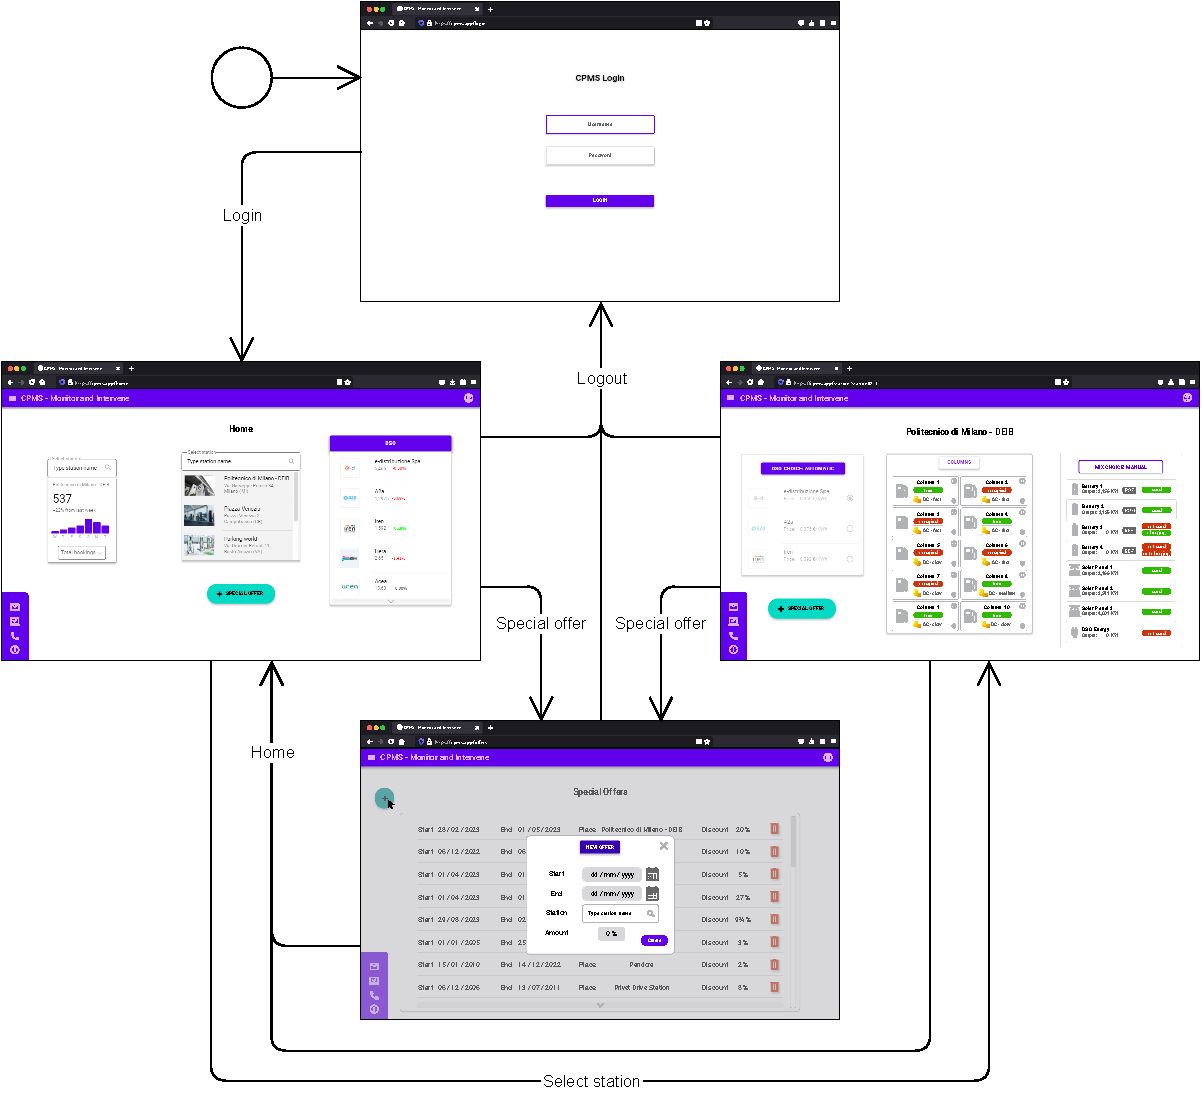
\includegraphics[width=\columnwidth]{./images/connections/cpms}
    \caption{the connections between the various interfaces.}
\end{figure}
